\documentclass[a4]{book}
\usepackage{listings}
\usepackage[T1]{fontenc}
\usepackage{courier}
\usepackage[utf8]{inputenc}
\usepackage[italian]{babel}
\usepackage{hyperref}
\usepackage{listings}
\usepackage{color}
\usepackage{graphicx}
\fontsize{7mm}{6mm}

\definecolor{mygreen}{rgb}{0,0.6,0}
\definecolor{mygray}{rgb}{0.5,0.5,0.5}
\definecolor{mymauve}{rgb}{0.58,0,0.82}
	
\lstset{ %
	backgroundcolor=\color{white},   % choose the background color; you must add \usepackage{color} or \usepackage{xcolor}
	basicstyle=\footnotesize,        % the size of the fonts that are used for the code
	breakatwhitespace=false,         % sets if automatic breaks should only happen at whitespace
	breaklines=true,                 % sets automatic line breaking
	captionpos=b,                    % sets the caption-position to bottom
	commentstyle=\color{mygreen},    % comment style
	deletekeywords={...},            % if you want to delete keywords from the given language
	escapeinside={\%*}{*)},          % if you want to add LaTeX within your code
	extendedchars=true,              % lets you use non-ASCII characters; for 8-bits encodings only, does not work with UTF-8
	frame=single,	                   % adds a frame around the code
	keepspaces=true,                 % keeps spaces in text, useful for keeping indentation of code (possibly needs columns=flexible)
	keywordstyle=\color{blue},       % keyword style
	language=C,                 % the language of the code
	otherkeywords={*,...},           % if you want to add more keywords to the set
	numbers=left,                    % where to put the line-numbers; possible values are (none, left, right)
	numbersep=5pt,                   % how far the line-numbers are from the code
	numberstyle=\tiny\color{mygray}, % the style that is used for the line-numbers
	rulecolor=\color{black},         % if not set, the frame-color may be changed on line-breaks within not-black text (e.g. comments (green here))
	showspaces=false,                % show spaces everywhere adding particular underscores; it overrides 'showstringspaces'
	showstringspaces=false,          % underline spaces within strings only
	showtabs=false,                  % show tabs within strings adding particular underscores
	stepnumber=2,                    % the step between two line-numbers. If it's 1, each line will be numbered
	stringstyle=\color{mymauve},     % string literal style
	tabsize=2,	                   % sets default tabsize to 2 spaces
	title=\lstname                   % show the filename of files included with \lstinputlisting; also try caption instead of title
}


\begin{document}

\begin{titlepage}
\begin{titlepage}
	\centering
	
\includegraphics[width=0.5\textwidth]{Alisea}\par\vspace{1cm}
	{\scshape\LARGE Università degli Studi di Parma \par}
	\vspace{1cm}
	{\scshape\Large Dipartimento di Informatica\par}
	\vspace{1.5cm}
	{\huge\bfseries Alisea\par}
	\vspace{2cm}
	{\Large\itshape Ivan Bergonzani e Gabriele Etta\par}
	
	\vfill
	

	{\large \today\par}
\end{titlepage}
\end{titlepage}


\tableofcontents

\chapter{Prefazione}
La seguente relazione vuole descrivere il lavoro svolto per la realizzazione del progetto richiesto all'interno del corso di Reti di Calcolatori. A seguire, verranno descritti tutti gli ambiti affrontati nello sviluppo, mettendo in evidenza sia gli aspetti più organizzativi, come la metodologia di lavoro utilizzata, che aspetti più tecnici relativi alle varie componenti dell'applicazione. Per quest'ultimo aspetto, vista la natura molto tecnica dell'applicazione, si è preferito fornire una descrizione intuitiva del funzionamento senza scendere a dettagli implementativi per ogni sua singola parte, rimandando al progetto vero e proprio nel caso si volesse approfondire ulteriormente. \\ \\
\textbf{Disclaimer: }il progetto fa riferimento allo streaming di video, senza riferirsi in alcun modo all'utilizzo di contenuti multimediali protetti da copyright. Le classi, i metodi e le relazioni che contengono al loro interno la parola \textit{film} sono da considerarsi a puro titolo d'esempio.
\chapter{Introduzione}

Alisea è un progetto nato con lo scopo di creare un'applicazione che permetta la visualizzazione di contenuti multimediali, principalmente di tipo audiovisivo, mediante la tecnica dello \textit{streaming} che sfrutta a sua volta il protocollo \textit{Bit Torrent} e la relativa architettura \textit{Peer to Peer (P2P)}. Il lavoro è stato realizzato seguendo una metodologia di sviluppo di tipo Agile, con vantaggi relativi alla gestione del lavoro e alla qualità del codice, facendo uso  delle più recenti tecnologie e strumenti messi a disposizione da Microsoft in modo tale da avere un'infrastruttura il più possibile omogenea ed efficiente sia dal punto di vista delle performance che dal punto di vista della qualità del codice. L'applicazione nella sua totalità è composta da:

\begin{itemize}
	
	\item \textbf{Un client} sviluppato mediante l'uso delle \textit{Universal Windows App} in modo tale da poter essere eseguito in ogni piattaforma che supporti Windows 10.
	\item \textbf{Una web application} sviluppata in \textit{ASP.NET MVC} che ha il compito di ospitare il sito web e di fare da Middle Layer ricevendo le richieste dall'applicazione mediante l'uso di API appositamente create e comunicando con il database trasferendo dati da entrambe le parti.
	\item \textbf{Un database remoto} basato su SQL Server 2012 per poter tenere traccia delle informazioni relative ai video.
	\item \textbf{Un database locale} basato su SQLite per poter tenere traccia di tutte le preferenze dell'utente verso i video.
	  
\end{itemize}
E' possibile visitare il sito del progetto all'indirizzo: \url{http://aliseamiddleservice.azurewebsites.net }


\chapter{Software utilizzati all'interno del progetto}

All'interno del progetto sono stati utilizzati diversi software e strumenti che verranno descritti in forma generale nella lista sottostante per poi essere ripresi in modo specifico nelle sezioni della relazione che ne hanno usufruito. E' stato utilizzato:

\begin{itemize}
	\item \textbf{Slack: }è uno strumento per la comunicazione all'interno di team lavorativi mediante l'uso di chat. Esso offre la possibilità di istituire dei gruppi di lavoro che possono creare canali di comunicazione al suo interno secondo i diversi ambiti lavorativi con la possibilità di integrare plugin esterni. Nel nostro caso ad esempio, è stato possibile integrare un canale del team chiamato \textit{repository - info} con un plugin di Visual Studio Team Services in modo tale che, ogniqualvolta uno sviluppatore inseriva del nuovo codice all'interno della repository, il plugin mandava un messaggio automatico all'interno del canale in questione informando tutti gli utenti di una nuova azione di \textit{push} da parte di uno sviluppatore con il relativo messaggio e con la possibilità di vedere quali parti di codice sono state modificate nelle diverse unità di traduzione.
	
	\begin{figure}[!h]
		\centering
		\caption{Un esempio di messaggi mandati dal Bot riguardante i nuovi commit all'interno della repository.}
		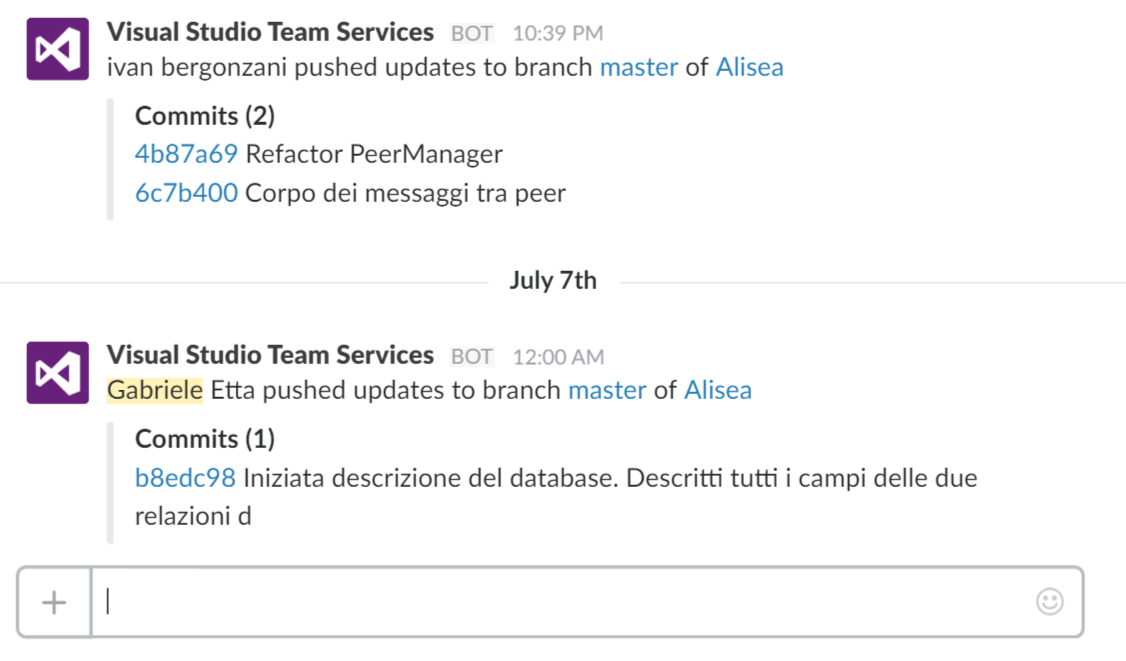
\includegraphics[scale=0.5]{slack}
		\medskip
		\small
	\end{figure}
	
	\item \textbf{Visual Studio Team Services:} strumento per la gestione di team online che offre supporto allo sviluppo secondo metodologie \textit{agile} offrendo una repository con cui condividere il codice a tutti gli utenti del team utilizzando un software di configuration management come \textit{Git} o \textit{TFS}.
	
	\item \textbf{Visual Studio Community 2015:} IDE di Microsoft per lo sviluppo dell'applicazione. Grazie ad esso è stato possibile sviluppare un prodotto eseguibile su tutti i dispositivi Windows grazie al framework \textit{Universal Windows Platform}
	
	\item \textbf{Visual Studio Express per Web:} IDE di Microsoft per lo sviluppo di applicazioni web. Esso è stato necessario per la creazione di tutto il backend dell'applicazione.
	
	\item \textbf{Microsoft Azure: }\textit{IAAS (Infrastructure As A Service)} di Microsoft per la creazione e la gestione di un sistema di cloud computing o per l'utilizzo di normali funzionalità a lato server come l'hosting di un sito o di un database. Nel nostro caso è stato d'aiuto per poter creare il sito dell'applicazione, il suo database e per poter hostare la \textit{web application} contenente tutte le API che andranno ad interrogare il database per inserire / prelevare dati.
	
	\item \textbf{SQL Server Management Studio:} software di Microsoft per la gestione di database basati su SQL Server. Grazie ad esso è stata possibile la gestione e la modifica del database presente sul server offerto da Azure.
\end{itemize}

\chapter{Metodologia di sviluppo utilizzata}
La metodologia di sviluppo utilizzata nel corso del progetto è ricercabile all'interno del framework \textbf{Scrum}. Con esso si intende un framework per lo sviluppo software basato sulla metodologia \textit{Agile} che introduce le seguenti novità al classico sviluppo \textit{waterfall}:

\begin{itemize}
	\item \textbf{Sviluppo iterativo ed incrementale:} lo sviluppo non è più diviso in fasi distinte tra loro, favorendo un'iterazione continua tra di esse mano a mano che l'applicazione prendeva forma. Così facendo si era portati a produrre poco codice alla volta ma continuamente testato e funzionante, e in caso di problemi di tipo progettuale era più facile eseguire un \textit{rollback} strutturale dell'applicazione rinunciando ad una mole di nuove modifiche molto ridotta.
	\item \textbf{Suddivisione del lavoro in finestre temporali (sprint):} il periodo di sviluppo all'interno del progetto era suddiviso in intervalli temporali chiamati \textit{sprint}: all'interno di essi venivano inizialmente definiti dei \textit{task} che corrispondevano all'atto di implementazione vero e proprio degli elementi e delle features dell'applicazione, che prendono il nome di \textit{Product Backlog}.
	\item \textbf{Tracciabilità continua dello stato del lavoro:} all'interno di ogni sprint, ciascun task era visibile all'interno di un'apposita tabella chiamata \textit{Kanban board}. Essa è formata generalmente da quattro colonne rappresentanti lo stato assumbile da ciascun task. Nella fattispecie:
	
	\begin{itemize}
		\item \textbf{Approvati:} colonna contenente tutti i \textit{task} di ciascun \textit{Product Backlog} (che da ora in poi chiameremo PB) che sono stati approvati per essere sviluppati nello sprint in esame.
		\item \textbf{Sviluppo:} colonna contenente tutti i task \textit{task} in sviluppo attuale.
		\item \textbf{In testing:} colonna contenente tutti i task in fase di testing. Nella nostra applicazione non è stata inserita assumendo però che ogni task per considerarsi completato debba essere prima testato con successo.
		\item \textbf{Completati: } colonna contenente tutti i task sviluppati e testati.
	\end{itemize}
	
	\begin{figure}[!h]
		\begin{center}
		\caption{Un esempio di Kanban board con i relativi task in stati diversi. }
		\centering
		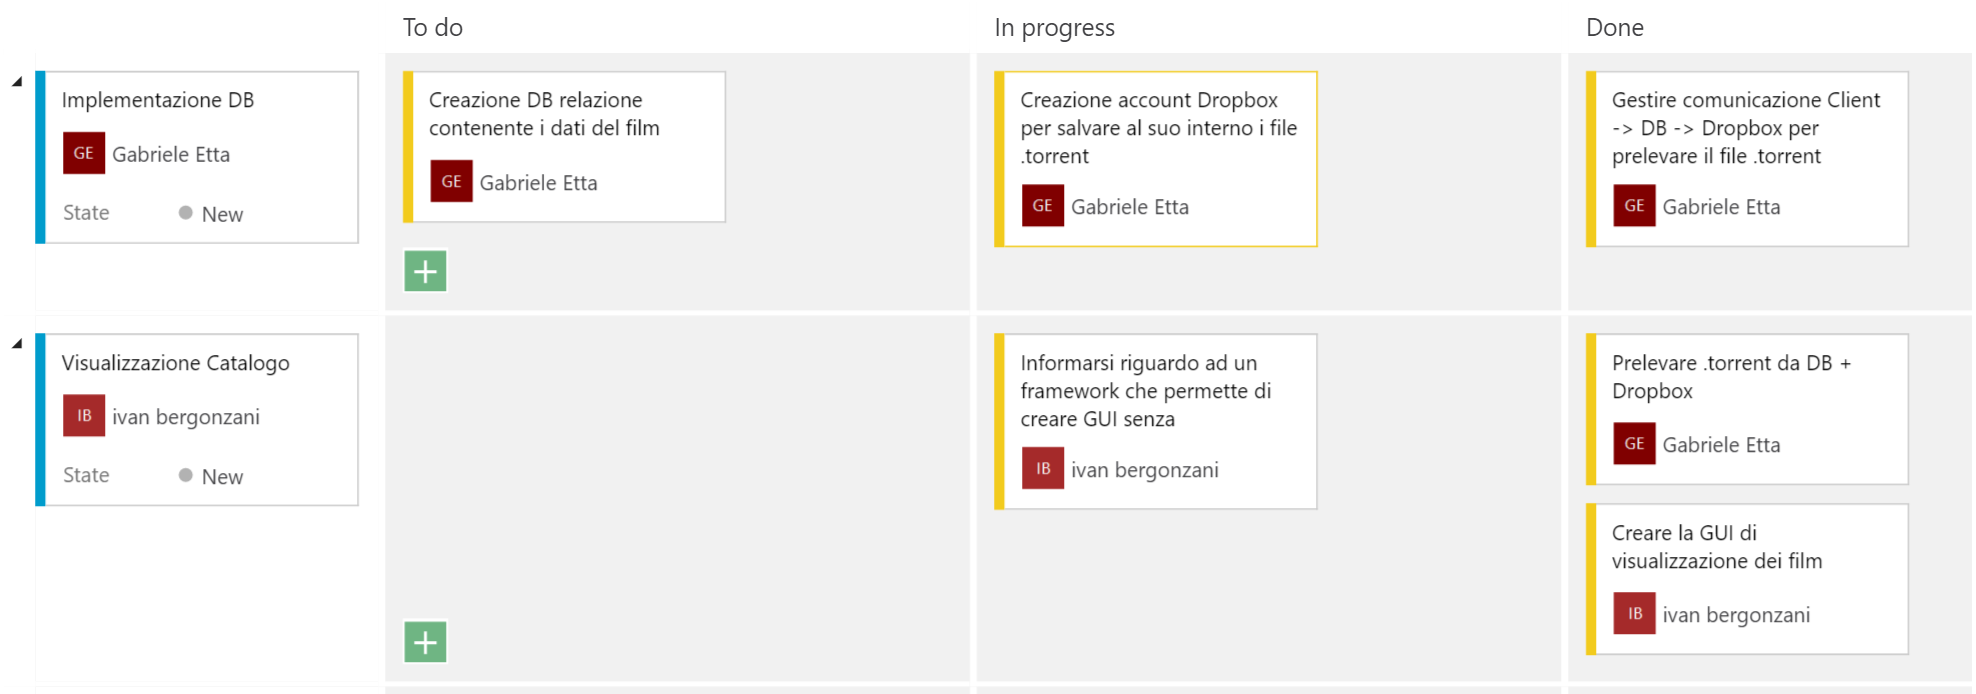
\includegraphics[scale=0.5]{backlog}
		\medskip
		
		\end{center}
	\end{figure}
	
	Dall'immagine si può intuire come questa metodologia di svilupp porti ad avere tanti piccole funzionalità testate e funzionanti preferendole a parti monolitiche di dimensioni considerevoli, la cui integrazione con l'applicazione può risultare in bug e problemi di una certa entità. Questo vantaggio è apprezzabile sul lungo termine del processo di realizzazione in cui la presenza molto ridotta di bug e dipendenze tra componenti fa si che si possa dedicare più tempo allo sviluppo che al \textit{bug fixing}.
	
	\item \textbf{Comunicazione continua all'interno del gruppo:} lo SCRUM, e in generale le metodologie agili, mettono al primo posto l'interazione fra individui. Questa caratteristica è stata ripresa anche nel corso del nostro progetto istituendo riunioni giornaliere, chiamate \textit{daily meeting}, in cui ogni membro del gruppo informava l'altro su che cosa ha fatto, farà e sta facendo con le relative problematiche di tipo tecnico e non. In questo modo ognuno di noi era al corrente della situazione lavorativa dell'altro, migliorando la cooperazione e la visione d'insieme a livello di applicazione.\\
\end{itemize}

Questa metodologia di sviluppo è stata implementata in modo efficace ed efficiente grazie ad uno strumento web citato precedentemente, chiamato \textbf{Visual Studio Team Services}. Esso si propone come un gestore di team prevalentemente di tipo agile, gratis per gruppi inferiori alle 5 persone: grazie ad esso è stato possibile avere implementati tutti gli strumenti per poter concretizzare tutti i punti descritti in precedenza, con la possibilità aggiuntiva di poter creare una repository di tipo \textit{Git} o \textit{TFS} per poter centralizzare il codice.
\chapter{Il backend: Alisea Middle Service}

Il progetto, oltre al client vero e proprio, si compone di un secondo elemento, il backend, chiamato \textit{Alisea Middle Service}. Da come si può intuire dal nome, esso funge da \textit{middle layer} tra l'applicazione ed il database instaurando un'architettura di tipo RESTful in cui l'applicazione, per prelevare tutte le varie tipologie di dato relativi ai video, dovrà contattare questo servizio mediante l'utilizzo di API preposte ai vari scopi perseguibili, con la conseguente risposta in formato JSON . La scelta di utilizzare questa architettura è caratterizzata dai seguenti vantaggi: \newline
\begin{itemize}
	\item \textbf{Richiesta computazionale ridotta da parte del client} in quanto dovrà solamente inviare e ricevere dati da/verso il backend per mezzo di chiamate HTTP, la cui risposta è codificata in JSON rendendo la comunicazione ancora più snella in quanto non sono necessarie decodifiche particolari della risposta.
	\item \textbf{Database e web application sono eseguiti su un server appartenente alla piattaforma Azure di Microsoft}. Questo, per come è definita l'infrastruttura, assicura la ridondanza geografica dei servizi, un certo livello di qualità qualità delle prestazioni inglobando al tempo stesso una metodica di \textit{weak scaling} in caso di un numero di richieste elevato.
	\item \textbf{Architettura di tipo \textit{three layer architecture}} per una maggiore \textit{fault tollerance} in quanto si hanno più punti di criticità anzichè uno centralizzato nel caso in cui il progetto avesse perseguito un'architettura di tipo \textit{client server}. \newline
\end{itemize}


\newpage
\section{Tecnologie e strumenti utilizzati}
Le tecnologie e gli strumenti utilizzati per la realizzazione del backend, comprensivi di database, sono:

\begin{itemize}
	\item \textbf{Microsoft Azure}
	\item \textbf{ASP.NET MVC}
	\item \textbf{Entity Framework: Code First!}
	\item \textbf{Microsoft SQL Server}
	\item \textbf{SQLite}
	\item \textbf{LINQ}	
\end{itemize}

Vediamo quindi ciascuna di esse nel dettaglio. \newline
\subsection{Microsoft Azure}
Microsoft Azure è un sistema operativo di Microsoft nato per supportare \textit{Windows Azure Platform}. Essa è stata scelta come piattaforma per il backend in quanto mette a disposizione caratteristiche interesasnti come il \textit{cloud computing}, la ridondanza geografica dei servizi creati al suo interno e un'architettura \textit{SOA (Service Oriented Architecture)}: quest'ultimo punto è di vitale importanza in quanto grazie ad esso è stato possibile gestire un database Microsoft SQL Server e creare un'applicazione web in ASP.NET senza che l'interoperabilità e l'integrità venissero intaccate.
Di norma, l'usufrutto dei servizi messi a disposizione dalla piattaforma è a pagamento, ma grazie a licenze particolari di tipo \textit{Dreamspark} è stato possibile poter avere accesso ad alcune sue funzionalità gratis, tra cui la possibilità di creare un database o di hostare una web application.

\subsection{ASP.NET MVC}

ASP.NET MVC è un framework di tipo Model-View-Controller sviluppato da Microsoft in aggiunta ad ASP.NET, dando la possibilità di creare Web Application così strutturate:

\begin{itemize}
	\item \textbf{Model:} contiene il modello dei dati, che nel nostro caso avrà al suo interno tutte le classi riferite alle diverse relazioni presenti sia nel database locale \textit{SQLite} che in quello su Azure basato su \textit{SQL Server}.
	\item \textbf{View:} contiene il codice HTML che da vita all'interfaccia utente. Nel nostro caso ci siamo limitati semplicemente a modificarlo per puri scopi presentativi.
	\item \textbf{Controller:} contiene tutta la logica di business dell'applicazione, che nel nostro caso faceva riferimento alla gestione vera e propria dei metodi associati alle API richiamate dall'applicazione, con i relativi routing in modo tale da poter associare ad ognuna di esse un URL univoco.	
\end{itemize}

\subsection{Entity Framework: Code First!}

\textit{Entity Framework : Code First!} è un approccio al design dei database relazionali figlio di \textit{Microsoft Entity Framework}. Con l'approccio \textit{Code first} è possibile creare un database partendo dalla programmazione delle singole classi a livello codice facendo in modo che il framework le "traduca" in relazioni vere e proprie, mappando i diversi tipi di dato e vincoli presenti da codice. Sebbene nel nostro contesto non sia presente una struttura complessa del database, questa metodica permette di avere una gestione più orientata alle singole componenti rispetto ad una visione classica in cui si generalmente è portati a definire tutta la struttura del database per poi passare all'implementazione concreta. Il vantaggio che si può trarre è quindi quello di una maggiore facilità di integrazione a livello codice, permettendo al tempo stesso modifiche più rapide un minor numero di operazioni sui dati inseriti o prelevati.


\subsection{Microsoft SQL Server}
Microsoft SQL Server, utilizzato nella versione 2012, è un RDBMS \textit{(Relational Database Managament System)} utilizzato all'interno del progetto per fornire un supporto alla memorizzazione di tutte le informazioni inerenti ai video e alle sue possibili categorie. Le diverse peculiarità e caratteristiche verranno mostrate mano a mano che verranno descritti i suoi ambiti di utilizzo. Per poter interagire con il database presente su un apposito server all'interno di Azure, è stata necessaria l'installazione del software \textit{SQL Server Management Studio} al fine di poter gestire tutti i suoi aspetti.


\subsection{SQLite}
SQLite è una libreria software scritta in linguaggio C che implementa un RDBMS incorporabile all'interno di applicazioni. Esso permette di creare basi di dati presenti in un unico file, traendo giovamento dalla sua compatezza, velocità e dal fatto che implementi transazioni ACID. Nel nostro caso, esso è stato utilizzato come al fine di implementare una sorta di registro per poter teneer traccia di tutti gli apprezzamenti effettuati dell'utente rispetto ai video, evitando così di dover scambiare dati di interesse locale con il server remoto..

\subsection{LINQ}
LINQ è una componente del Framework di Microsoft .NET che aggiunge ai linguaggi appartenenti di questa famiglia la possibilità di effettuare interrogazioni al database lavorando su oggetti. Questa scelta, preferendo la sintassi classica delle interrogazioni SQL, è dovuta al fatto che in questo modo è possibile abbracciare in modo migliore la filosofia d'uso introdotta da Entity Framework in cui tutto ciò che è relazionato al database deve essere effettuato via codice, migliorando anche le performance dal momento che una query dinamica scritta in SQL classico è sicuramente meno performante in termini di velocità di esecuzione rispetto all'utilizzo di \textit{properties} e metodi offerti dal framework stesso.

\section{Gestione e struttura del database}
Alisea è un'applicazione che fa uso delle basi di dati, ovvero di un insieme strutturato di dati le cui informazioni contenute seguono un particolare modello logico detto \textit{modello relazionale}. In questo tipo di modello, tutti i dati sono rappresentati come delle relazioni dal punto di vista matematico che possono essere manipolate mediante gli operatori dell'algebra relazionale o del calcolo razionale. La struttura base sui cui è fondato questo modello è composta da:
\begin{itemize}
	\item \textbf{Attributi}: riconducibile ad un campo dati (colonna).
	\item \textbf{Tipo di dato e dominio:} specifica l'insieme di valori che può assumere un determinato attributo.
	\item \textbf{Valore per ciascun attributo}.
	\item \textbf{Record:} insieme non ordinato di valori assunti dagli attributi.
\end{itemize}

Ogni base di dati, per essere correttamente implementata e gestita, fa uso di un particolare tipo di software chiamato \textit{Database Management System (DBMS)} che nel nostro contesto assume il nome particolare di \textit{RDBMS} in quanto si ha a che fare con basi di dati relazionali. All'interno del nostro progetto sono stati usati due tipi di RDBMS come precedentemente enunciato, ovvero \textit{Microsoft SQL Server}, nella versione 2012, e \textit{SQLite}. Per ognuno di essi, andiamo a descrivere la struttura delle relazioni che contengono, con le relative considerazioni.

\subsection{Gestione del catalogo dei video e delle relative categorie: Microsoft SQL Server}

Dal momento che l'applicazione ha come obiettivo principale quello di permettere lo streaming di video a tutti gli utilizzatori, è stato necessario l'utilizzo di un database centralizzato accessibile da ogni locazione geografica, chiamato per originalità \textit{Alisea}. Esso comprende le seguenti due relazioni:

\begin{itemize}
		\item \textbf{Films}: è la relazione che conterrà tutti i record con le informazioni relative ai video. Essa è formata dai seguenti attributi:
		\begin{itemize}
			\item \textbf{ID:} di tipo \textit{int} e non nullo, rappresenta il codice univoco di ciascun video. Questo campo verrà popolato con un numero automatico successivo a quello relativo all'ultimo record inserito. La scelta di utilizzare un intero a 32 bit è data dal fatto che si è supposto di generalizzare questa applicazione per un possibile uso globale, anche se per i nostri scopi sarebbe stato sufficiente utilizzare un \textit{tinyint} a 8 bit, per un totale di 255 video massimi archiviabili.
			
			\item \textbf{Title: } di tipo \textit{nvarchar(100)} e non nullo, è la chiave primaria della relazione e rappresenterà il nome del regista del video. La scelta di utilizzare \textit{nvarchar} e non \textit{varchar} è dovuta al fatto che il primo tipo permette di salvare stringhe testuali in formato \textit{Unicode} in quanto per registi di nazionalità particolari (ad esempio occidentali) è possibile dover inserire caratteri non presenti nello standard \textit{ASCII}. Ragionamenti simili a questo sono stati applicati in tutti gli altri campi testuali dello stesso tipo.
			
			\item \textbf{Length: } di tipo \textit{smallint} e non nullo, rappresenta la lunghezza del video.
			
			\item \textbf{ReleaseDate: } di tipo \textit{date}, rappresenta la data di uscita del video.
				
			\item \textbf{InsertDate: } di tipo \textit{date}, rappresenta la data di inserimento del video all'interno del database.
			
			\item \textbf{Actors:} di tipo \textit{nvarchar(500)} e non nullo, rappresenta la lista di tutti gli attori principali che hanno preso parte al video.
			
			\item \textbf{Category}: di tipo \textit{nvarchar(100)}, non nullo, rappresenta la categoria del video che fa riferimento alla relazione \textit{Categories} in cui sono salvati tutte le loro possibili categorie.
			
			\item \textbf{FilmDescription}: di tipo \textit{nvarchar(max)} e non nullo, contiene la trama del video. La scelta di non mettere un limite superiore alla lunghezza di questo campo è dovuta al fatto che la trama possa avere lunghezze impredicibili, optando per sacrificare performance e spazio in favore di una \textit{user experience} migliore.
			
			\item \textbf{ImagePath, ThemePath, TorrentLink:} sono tutti e tre dei campi testuali di tipo \textit{nvarchar(500)} contenenti rispettivamente i link alla locandina del video, allo sfondo presente nella sua pagina dei dettagli e al link del torrent. La scelta di non sostituire i primi due campi con uno di tipo \textit{BLOB} è dettata chiaramente da ragioni di spazio e performance: nella sottoscrizione Dreamspark di Microsoft con cui è stato realizzato il progetto, il database può essere al più di 32MB e pertanto si è scelto di tenere dei link diretti alle immagini scaricabili poi da client. Inoltre, le operazioni di scrittura rispetto ad esso sono più inefficienti dell'alternativa utilizzata, e i backup del database possono aumentare in modo esponenziale in termini di spazio.
			
			\item \textbf{Thumbs:} di tipo \textit{smallint} e non nullo, è il contatore dei "Like" lasciati dagli utenti al video. Di default esso parte da 0.
			
			\item \textbf{Weekly:} di tipo \textit{smallint} e non nullo, è il contatore settimanale dei "Like" lasciati dagli utenti al video. Di default esso parte da 0 e ogni lunedì viene azzerato.
			
			\item \textbf{Visualizations: } di tipo \textit{smallint} e non nullo, è il contatore delle visualizzazioni di un video.
		\end{itemize}
		
		\item \textbf{Categories:} relazione contenente il nome di tutte le possibili categorie di video supportate dall'applicazione. Essa dispone di un solo attributo, chiamato \textbf{Name}, di tipo \textit{nvarchar(100)}, non nullo e chiave primaria della relazione, che rappresenta il nome della categoria.
		
\end{itemize}

La scelta di utilizzare l'attributo \textit{Title} come chiave primaria è data dal fatto che SQL Server introduce di default un \textbf{indice clustered} per tale attributo, facendo si tutti i record all'interno di tale relazione vengano ordinati lessicograficamente. Un \textbf{indice clustered}, per definizione, è una struttura dati rappresentata da un albero bilanciato che fa riferemento ad uno o più attributi in modo tale da garantire un ordinamento di tutti i nodi. Questa caratteristica fa sì che nella ricerca di un record secondo un criterio basato sui campi indicizzati, il motore di esecuzione della query non dovrà più scandirli uno per uno ma dovrà solamente visitare l'albero restringendo mano a mano l'intervallo di ricerca fino a ritornare il result set desiderato.

\begin{figure}

\caption{Struttura di un indice clustered e non clustered a confronto.}
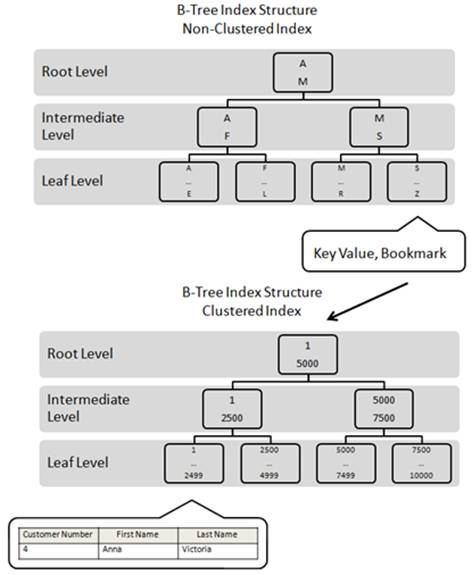
\includegraphics{index}
\medskip
\small
\end{figure}

In aggiunta a questo, un \textit{indice clustered} contiene all'interno dei suoi nodi i record veri e propri, a differenza degli \textit{indici non clustered} che invece memorizzano i puntatori ai record. Il vantaggio di tale scelta all'interno dell'applicazione si ha dal momento che la maggior parte delle query eseguite dal client hanno dei criteri di ricerca basati sul titolo del video. Indicizzandolo quindi è possibile ridurre i tempi di ricerca dei record voluti migliorando la velocità di comunicazione. \newline

\subsection{Gestione dei video preferiti dall'utente e delle relative preferenze da parte dell'utente: SQLite}
L'utente, all'interno dell'applicazione, ha la possibilità di fornire un parere sui video mediante la pressione di opportuni tasti nella sua pagina di descrizione o in alternativa può aggiungerlo alla lista dei suoi video preferiti. Poichè entrambe le scelte sono rappresentabili mediante uno storico di interesse relativo all'utente, si è preferito creare un database locale atravverso l'uso dell' RDBMS \textit{SQLite} in favore di uno remoto basato su SQL Server. I motivi di tale scelta sono dettati dalle performance, esposti nel paragrafo precedente, integrandosi in modo migliore con la natura dinamica e snella delle Universal Windows App. Vediamo quindi le relazioni ospitate al suo interno:

\begin{itemize}
	\item \textbf{Favorites}: contiene i riferimenti ai video che l'utente ha aggiunto ai preferiti. Essa si compone di un unico attributo di tipo intero, \textbf{ID} che è anche chiave primaria dell'applicazione, i quali poi diventeranno i criteri di ricerca per prelevare tutte le informazioni ad esso associate in modo tale da poter essere visualizzate nella schermata apposita dell'applicazione.
	\item \textbf{Likes}: contiene tutte le informazoni riguardanti i video a cui l'utente ha fornito un giudizio positivo o negativo. Questa relazione si compone dei seguenti campi:
	\begin{itemize}
		\item \textbf{idFilm:} chiave primaria di tipo \textit{int}, contiene il codice del video al quale l'utente ha espresso un giudizio.
		\item \textbf{like}: di tipo \textit{bool}, se impostata a \textit{true} indica che l'utente ha apprezzato il video, mentre \textit{false} è il valore neutro di default.
		\item \textbf{dislike}: anch'esso di tipo \textit{bool}, ha la stessa semantica del campo soprastante con la differenza che un suo valore a \textit{true} indica l'apprezzamento dell'utente al video. Sia il campo like che dislike non possono essere contemporaneamente impostati a \textit{true}.
	\end{itemize}
\end{itemize}


\section{Creazione dei database}

Definita la struttura dal punto di vista relazionale, cominciamo ad illustrare il ciclo di vita dei due database partendo dalla loro creazione.

\subsection{Microsoft SQL Server:}

Per tutta la gestione del database remoto su SQL Server è stato utilizzato il framework \textit{Entity Framework: Code First!}: esso, come accennato ad inizio capitolo, permette di creare ed interagire una base di dati da codice senza l'ausilio del linguaggio SQL ma facendo affidamento a delle classi create ad hoc, utilizzando chiaramente particolari meccaniche messe a disposizione dallo strumento stesso. Entriamo quindi nel dettaglio: per creare la relazione \textit{Films} e \textit{Categories} sono state create le rispettive classi \textit{Film} e \textit{Category} all'interno del progetto di backend di tipo ASP.NET MVC, precisamente nella cartella \textit{Model} dove sonopresenti appunto i nostri modelli di riferimento su cui eseguiremo tutte le operazioni. Mostriamo a seguire le dichiarazioni delle due classi:

\lstset{language=[Sharp]C}
\begin{lstlisting}


	  public class Film
	  {
		  public int ID { set; get; }
		  public string Title { set; get; }
		  public string Director { set; get; }
		  public short Length { set; get; }
		  public DateTime ReleaseDate { set; get; }
		  public DateTime InsertDate { set; get; }
		  public string Actors { set; get; }
		  public string Category { set; get;}
		  public string FilmDescription { set; get; }
		  public string ImagePath { set; get; }
		  public string ThemePath { set; get; }
		  public string TorrentLink { set; get; }
		  public short Thumbs { set; get; }
		  public short WeeklyThumbs { set; get; }
		  public short Visualizations { set; get; }
	  }
	
	
	
\end{lstlisting}

\lstset{language=[Sharp]C}
\begin{lstlisting}
public class Category
{
	public string Name{ get; set;}
}
\end{lstlisting}


Dalla definizione della classe si può evincere che i tipi dei vari campi corrispondono esattamente a quelli degli attributi sul database: non è stato necessario eseguire una mappatura manuale in quanto \textit{Entity Framework} se ne è occupato al posto nostro. Si può anche notare che non sono stati definiti vincoli di nessun tipo: questo perchè siamo ancora distanti dalla loro trasformazione in relazioni, evitando quindi di introdurre dipendenze funzionali che precluderebbero l'utilizzo di esse al di fuori del contesto attuale relativo al database. \newline
Definite la classi che fungeranno da relazioni, è necessario renderle tali eseguendo delle \textbf{migrazioni}. Una migrazione in \textit{Entity Framework} è un modo per apportare le modifiche dei modelli direttamente su database. Nel caso come il nostro in cui abbiamo a che fare con la prima migrazione del progetto, il framework dedurrà questa cosa e creerà automaticamente dei costrutti riconducibili alla creazione della tabelle. Per poter effettuare una migrazione, è necessario prima di tutto abilitarle dalla console di \textit{NuGet} mediante il comando \texttt{Enable - Migrations}, seguito dal comando di creazione \texttt{Add-Migration NomeMigrazione}. Una volta lanciato, il framework creerà automaticamente una classe parziale derivata da \textit{DBMigration} che nel nostro caso è la seguente:

\begin{lstlisting}
	
public partial class Inizio : DbMigration
{
	public override void Up()
	{
		
		CreateTable(
		
			"dbo.Categories",
			c => new
			{
			
			Name = c.String(maxLength:100)
		}).PrimaryKey(c => c.Name);
		
		
		CreateTable(
			"dbo.Films",
			c => new
			{
				ID = c.Int(identity:true, nullable:false),
				Title = c.String(nullable:false, maxLength:100),
				Director = c.String(nullable:false),
				Length = c.Short(nullable:false),
				ReleaseDate = c.DateTime(nullable:false),
				InsertDate = c.DateTime(nullable:false),
				Actors = c.String(nullable:false, maxLength:500),
				Category = c.String(maxLength:100, nullable:false),
				FilmDescription = c.String(nullable:false),
				ImagePath = c.String(nullable:false),
				ThemePath = c.String(nullable: false),
				TorrentLink = c.String(nullable: false),
				Thumbs = c.Short(defaultValue:0),
				WeeklyThumbs = c.Short(defaultValue:0),
				Visualizations = c.Short(defaultValue:0),
			
			
			})
			.PrimaryKey(t => t.Title);
		}
	
	
	
	public override void Down()
	{
		// Empty.
	}
}
\end{lstlisting}

Ogni migrazione ha due metodi al suo interno: \textbf{Up()} e \textbf{Down()}: il primo fa riferimento ad una situazione in cui le modifiche dovranno essere apportate al database, la seconda al momento in cui dovrà avvenire l'operazione inversa partendo però dal database. In questo caso, poichè vogliamo creare un database senza volerlo eliminare nel futuro, abbiamo modificato il codice svuotando il metodo \textit{Down}. Inoltre, abbiamo inserito manualmente tutti i vincoli di attributo e di dominio in modo tale da non dover eseguire una serie successive di modifiche da SQL. La sintassi utilizzata per eseguire queste operazioni è proprietaria del framework \textit{LINQ} di cui abbiamo già parlato in precedenza e che verrà ripresentata più volte all'interno del capitolo. \newline
Per poter apportare le modifiche sul server di Azure, è necessario lanciare da console il comando \texttt{Update-Database} che, facendo riferimento alla stringa di configurazione del nostro server in remoto, apporterà le modifiche su di esso.


\subsection{SQLite}
Per creare il database di SQLite, essendo locale all'utente, non siamo dovuti passare per il backend ma abbiamo agito dal client. Il procedimento è comunque analogo a quanto visto: abbiamo definito le classi di partenza necessarie, che in questo caso si chiamano \textit{Favorites} e \textit{Like}, nel modo seguente:

\begin{lstlisting}
 /// <summary>
 /// This class is used to create a localdb, using SQLite, to store all the favorite videos from the user.
 /// </summary>
 class Favorites
 {
	 /// filmID is the only column of the database, which is also a primary key, which will contain the id
	 /// of the films prefered from the user.
	 [PrimaryKey]
	 public int filmID { get; set; }
 }
\end{lstlisting}

\begin{lstlisting}

/// This class represent every video liked or disliked from the user. Everytime he presses the like or
/// dislike button in a video detail page, a new record is created with the correct value of like or dislike,
/// or instead there will be modified in order to reflect users actions. For each video, like and dislike button
/// can't have the same value.
class Like
{
	[PrimaryKey]
	public int idFilm { get; set; }
	public bool like {get; set;}
	public bool dislike { get; set; }
 
	public Like()
	{
		this.like = false;
		this.dislike = false;
	}
}
\end{lstlisting}

Poichè SQLite non offre un meccanismo di creazione di relazioni come quello di Entity Framework, è stato necessario definire tutti i vincoli necessari direttamente dalla classe. Il fatto che la chiave primaria sia l'ID del video non corrisponde a quanto mostrato nella creazione della relazione sul database remoto, ma si tratta di una scelta puramente indicativ< in quanto non c'è nessuna relazione vera e propria tra i due database secondo quegli attributi. Per creare il database in locale, all'interno della cartella di installazione dell'applicazione, si è fatto affidamento ad una classe apposita presente nel client adibita a tutte le operazioni che includono l'uso di un database, sia locale che remoto. Questa classe si chiama \textbf{DatabaseManager} di cui diamo la dichiarazione della sua interfaccia implementata, \textbf{IDatabaseManager}  con la descrizione dei suoi metodi (in inglese): \newline
\textbf{IDatabaseManager:}

\begin{lstlisting}
interface IDatabaseManager
{
	/// Retrieve a list of videos from database ordered by the number of thumbs, descendent.
	/// <returns>The list of the videos obtained.</returns>
	Task<List<Film>> GetTopFilm();
	
	/// Retrieve a list of videos from database ordered by their launch date, descendent.
	/// <returns>The list of the videos obtained.</returns>
	Task<List<Film>> GetNewFilm();
	
	/// Retrieve a list of videos from database ordered by the number of weekly thumbs, descendent.
	/// <returns>The list of videos obtained.</returns>
	Task<List<Film>> GetHotFilm();
	
	/// Retrieve a list of videos containing the string passed as parameter.
	/// <param name="searchToken">A string containing the name of the video or a part of it.</param>
	/// <returns>The list of the videos obtained.</returns>
	Task<List<Film>> SearchFilm(String searchToken);
	
	/// Retrieve a list containing all the video categories stored in the database.
	Task<List<FilmCategory>> GetFilmCategories();
	
	/// Given the name of the category, this method will return all the videos with that category.
	Task<List<Film>> GetFilmsFromCategory(string categoryName);
	
	/// Adds one thumb to the relative column of the video, specified with an id.
	/// <param name="filmID">The id of the video the user liked.</param>
	void AddThumbUp(int filmID);
	
	/// Subctract one thumb to the relative column of the video, specified with an id.
	/// <param name="filmID">The id of the video the user disliked.</param>
	void AddThumbDown(int filmID);
	
	/// Adds one visualization to the relative column of the video, specified with an id.
	/// <param name="filmID">The id of the video the user has viewed.</param>
	void AddVisualization(int FilmID);
	
	/// Check if database exists. If doesn't, then it will be created.
	/// <returns>true if the db and the tables are created, false otherwise.</returns>
	bool CreateLocalDatabase();
	
	/// Adding the video id into the favorites table.
	bool AddFavorite(int id);
	
	/// Retrieve a favorite from an ID, if exists.
	/// <returns>true if the video is found from the local favorites, false otherwise.</returns>
	bool GetFavorite(int filmID);
	
	/// Delete a favorite video from local database, given an ID.
	/// <returns>true if the favorite video was removed from the local db, false otherwise.</returns>
	bool removeFavorite(int filmID);
	
	/// Given the filmID, the method check if the video was previously liked or disliked in order to
	/// disable the related buttons on the page.
	/// <param name="filmID">the ID of the video.</param>
	/// <returns>1 if the video was previously liked, 2 if disliked, 0 if none of them.</returns>
	int GetLikeOrDislike(int filmID);
	
	/// Setting the like field of the video, identified with the ID, to true.
	/// <returns>true if the operation terminates correctly, false otherwise.</returns>
	bool addLike(int filmID);
	
	/// Setting the dislike field of the video, identified with the ID, to true.
	/// <returns>true if the operation terminates correctly, false otherwise.</returns>
	bool addDislike(int filmID);
	
	/// Obtaining the list of favorite videos stored in the local db.
	/// <returns>The row field of the favorite videos</returns>
	Task<List<Film>> GetFavoriteFilms();
}
\end{lstlisting}

Mostriamo dunque la prima definizione del metodo di cui si è parlato in precedenza riguardo alla creazione del database locale: \textbf{CreateLocalDatabase}. Questo metodo non farà altro che controllare se il database non è già stato creato e, in caso affermativo, creerà il database contenente le due tabelle partendo dalle classi mostrate in precedenza.

\begin{lstlisting}

 public bool CreateLocalDatabase()
 {
	 // Check if the db was already created.
	 if (File.Exists("dbo.alisea"))
	 {
		 Debug.Write("The db is already created.");
		 return false;
	 }
	 
	 // Creating the tables from the class, which will be 
	 // called just by inserting an object of their class.
	 this.conn.CreateTable<Favorites>();
	 this.conn.CreateTable<Like>();
	 
	 
	 return true;
 }
\end{lstlisting}

 La creazione del database è intrinseca alla creazione delle tabelle in quanto la variabile \textit{conn} è stata così definita nel costruttore della classe:
 
\begin{lstlisting}
	 string path = Path.Combine(Windows.Storage.ApplicationData.
	 Current.LocalFolder.Path, "dbo.alisea");
	 
	 this.conn = new SQLite.Net.SQLiteConnection(new
	 SQLite.Net.Platform.WinRT.SQLitePlatformWinRT(), path);
\end{lstlisting}

Ovvero, si posiziona all'interno della classe locale a dove l'app è stata installata e combina il suo percorso con quello del nome del database, stabilendo una connessione con esso che se usata per creare delle tabelle porterà prima alla creazione del database, nel caso non fosse presente.



\section{Comunicazione con i database}
Ora che i database sono stati creati, mostriamo come l'applicazione gestisce le diverse tipologie di comunicazioni con essi. Anche in questo caso facciamo distinzione tra i due database, elencando per ognuno di essi le operazioni in cui sono coinvolti.

\subsection{Modifica e lettura dei video e delle categorie: Microsoft SQL Server}
In via del tutto generale, dal momento che Alisea è un progetto che rispecchia una \textit{Three Tier Architecture} e poichè vogliamo alleggerire il client il più possibile in quanto eseguibile anche da dispositivi mobili, ogni operazione è costituita da una \textbf{chiamata formulata dal client verso la corrispondente API (web app)}, seguita da una \textbf{comunicazione tra web app e database}, ottenendo così i dati e seguendo il percorso inverso per ritornare la risposta. Attraverso la comunicazione con il database remoto è possibile fornire all'utente la lista di video con le relative categorie. Nello specifico, è possibile:

\begin{itemize}
	\item \textbf{Prelevare la lista delle categorie dei video:} in generale il client costruirà la richiesta HTTP, impostando come MIME-Type di risposta il formato JSON e indicando il link remoto alla web app con la relativa API che in questo caso è \texttt{api/Categories}. Poichè tutte le richieste remote hanno la stessa struttura, mostriamo un esempio di chiamata da client generale sostituendo le sole parti variabili:
	
	\begin{lstlisting}
		
List<Tipo> Nome = new List<Tipo>();
	
using (var client = new HttpClient())
{
	//Setting up the address of the service and the type of the response waited for. 
	client.BaseAddress = new Uri("http://aliseamiddleservice.azurewebsites.net");
	client.DefaultRequestHeaders.Accept.Clear();
	client.DefaultRequestHeaders.Accept.Add(new MediaTypeWithQualityHeaderValue("application/json"));

	// The api we want to call.
	HttpResponseMessage response = await client.GetAsync(NomeApi);


	//If the response is right, the string given as response will be parsed from
	JsonConvert object into Tipo.
	
	if (response.IsSuccessStatusCode)
	{
		string JSONResponse = await response.Content.ReadAsStringAsync();
		Nome = JsonConvert.DeserializeObject<List<Tipo>>(JSONResponse);
	}

return Nome;
}
	\end{lstlisting}
	
	Dalla web application, poichè rispecchia il formato MVC avremo un \textit{Controller} apposito per ogni classe creata precedentemente. Nel nostro caso ci ritroveremo quindi con le classi \textit{FilmsController} e \textit{CategoriesController} che implementano tutti i metodi eseguiti alla chiamata di una certa API che fa riferemento ad una relazione piuttosto che ad un altra, con le relative impostazioni di routing se necessarie. 

	\item \textbf{Prelevare tutti i video appartenenti ad una certa categoria:} mediante l'API \texttt{api/Films/Get/FilmsFromCategory/{category}} a cui il client dovrà passare come la categoria desiderata come parametro.
	
	\item \textbf{Prelevare gli ultimi video aggiunti:} mediante l'API \texttt{api/Films/NewFilms}, ordinati in modo decrescente partendo dall'ultimo aggiunto video.
	
	\item \textbf{Prelevare i video con più preferenze nell'arco della settimana:} mediante l'API \textit{api/Films/TrendingFilms}.
	
	\item \textbf{Prelevare i video più visualizzati in totale:} mediante l'API \texttt{api/Films/MostViewedFilms} che ritornerà una lista di video ordinata in modo decrescente in base al numero di visualizzazioni.
	
	\item \textbf{Prelevare un video dato il suo ID:} mediante l'API \texttt{api/Films/{filmID}} a cui è necessario fornire l'ID del video desiderato.
	
	\item \textbf{Prelevare tutti i video che contengono una determinata stringa:} mediante l'API \texttt{api/Films/Search/{title}}, implementa la ricerca di un video sfruttando il fatto che la relativa relazione sia indicizzata sull'attributo \textit{Title}.
	
	
	\item \textbf{Resettare i contatori settimanali delle visualizzazioni di tutti i video:} mediante l'API \texttt{api/Films/ResetWeeklyThumbs} che richiamata ad inizio di ogni settimana vuole simulare l'azzeramento del campo \textit{WeeklyThumbs} di tutti i record dei video.
	
	\item \textbf{Aggiungere una visualizzazione ad un video:} mediante l'API \texttt{api/Films/AddFilmVisualization/{idFilm}} che aggiunge una visualizzazione totale e settimanale in più al video identificato dall'ID passato come parametro.
	
	\item \textbf{Aggiungere un like o un dislike ad un video:} rispettivamente mediante le API \textit{api/Films/ThumbsUp/{idFilm}} e \texttt{api/Films/ThumbsDown/{idFilm}} che dato l'ID del video passato come parametro vanno ad aggiungere o sottrarre un'unità all'attributo relativo al valore totale degli apprezzamenti espressi per esso.
	

\end{itemize}

\subsection{Inserire video preferiti e apprezzamenti per essi: SQLServer}

Dal punto di vista del database locale, non avverrà nessuna interazione con il backend nonostante se ne stia parlando all'interno del suo capitolo. Procediamo quindi con il descrivere le operazioni svolte:

\begin{itemize}
	\item \textbf{Inserimento di un video preferito:} all'interno della relazione \textit{Favorites}, verrà salvato il solo ID del video che l'utente ha deciso di mettere tra i preferiti.
	\item \textbf{Modifica del valore relativo all'apprezzamento o meno di un video:} ogni volta che l'utente preme il tasto di apprezzamento o meno di un video, viene inserito un record che lo rappresenta all'interno della relazione \textit{Films} o se già presente vengono variati i campi \textit{Like} e \textit{Dislike} per rispecchiare lo stato attuale del giudizio espresso dall'utente in merito al video.
\end{itemize}

\chapter{Client Alisea: informazioni preliminari}
Il client consiste in un'applicazione UWP che permette, come accennato in precedenza, la navigazione tra gli elementi di un catalogo di contenuti multimediali e la successiva riproduzione. L'applicazione si divide principalmente in tre parti distinte: la comunicazione con il backend, per le richieste del catalogo multimediale, la comunicazione peer-to-peer, per l'ottenimento dei dati da riprodurre, e la parte grafica per mostare all'utente i contenuti ottenuti.\newline
Prima di addentrarsi nella struttura e nel funzionamento dell'applicazione Alisea analizziamo le caratteristiche che stanno alla base del progetto: lo sviluppo dell'applicazione ha reso infatti necessario l'analisi e l'utilizzo di diverse teconologie e protocolli:

\section{Tecnologie}
A seguire vengono illustrate velocemente le principali tecnologie sfruttate per la creazione del client Alisea.
\subsection{Universal Windows Platform}
Tramite la tecnologia Universal Windows Platform risulta possibile sviluppare applicazioni universali per l'ambiente Windows: questo significa che un'unica applicazione UWP può essere eseguita su tutti i dispositivi Windows 10 quali smartphone, pc desktop, notebook, console e prodotti 2 in 1.\newline
Chiaramente diversi dispositivi possiedono diverse caratteristiche: un esempio è dato dalla grandezza dello schermo che può variare da pochi pollici (smartphone) a diverse decine (Lavagne interattive). Nonostante il cuore dell'applicazione sia identico risulta comunque necessario adattare diversi dettagli ai dispositivi in modo da garantire la migliore \textit{user experience} possibile.\newline

\subsection{Codifica Bencode}
Il Bencoding è un metodo di rappresentazione dei dati derivato da XML. Utilizzato principalmente per la codifica dei file Torrent, supporta 4 tipi di dato: stringhe di byte, interi, liste e dizionari. Le liste e i dizionari possono contenere ognuno dei tipi di dato supportati senza limitazioni sulla quantità. Nello specifico:
\begin{itemize}

\item Le \textbf{stringhe di byte} vengono codificate nella forma \textbf{<lunghezza>:<dati>}. Il campo $lunghezza$ è un valore decimale codificato in ASCII e rappresenta l'effettiva lunghezza della stringa di byte mentre con il campo $dati$ si vuole indicare l'insieme di byte che forma la stringa.
\item I \textbf{numeri} vengono codificati nella forma \textbf{i<intero decimale codificato in ASCII>e} i cui delimitatori $i$,$e$ rappresentatno rispettivamente l'inizio e la fine del campo numerico. Un esempio è dato dai valori $-2$ e $3$ che sono codificati rispettivamente in $i-2e$ e $i3e$.
\item Le \textbf{liste} vengono codificate nella forma \textbf{l<contenuto della lista>e}. Il contenuto della lista può essere una sequenza di qualsiasi altro tipo di valori mostrati in precedenza, ovvero stringhe, interi, liste, dizionari. I valori $l$, $e$ definiscono l'inizio e il termine della lista stessa, mentre la sequenza \textbf{le} rappresenta la lista vuota.
\item I \textbf{dizionari} vengono codificati nella forma \textbf{d<Stringa Bencode>:<Valore Bencode>e}. Il contenuto è una sequenza di coppie chiave \textit{(stringa bencode)} e valori \textit{(valori bencode)}. Come per le liste, anche per esse il campo \textit{valore} può essere qualsiasi altro tipo bencode.\newline
\end{itemize}

\subsection{Programmazione asincrona, Async Task}
L'applicazione, considerato che fa del networking la sua componente principale, necessita di costrutti per poter eseguire parti di codice in modo indipendente e talvolta concorrenti. E' sufficiente individuare il thread dell'interfaccia grafica e le routine per lo scambio dei dati tra i dispositivi collegati: lo scenario comune prevede di mantenere l'applicazione sempre reattiva e quindi il thread UI non deve assolutamente bloccarsi a causa di altre funzionalità. La routine per lo scambio dati  quindi di essere eseguita eseguita in modo asincrono: a tale scopo sono utilizzati thread secondari eseguiti in background che spesso devono essere costruiti e gestiti direttamente dal programmatore. Per venire in contro a queste problematiche legate la gestione del codice asincrono, il linguaggio di programmazione C\# mette a disposizione le parole chiave \textbf{async} e \textbf{await} le quali permettono di utilizzare le risorse di .NET Framework o di Windows Runitime per la creazione di metodi asincroni.\newline
Segue un esempio di metodo asincrono:\newline
\begin{lstlisting}
async Task<int> AccessTheWebAsync()
{ 
	HttpClient client = new HttpClient();
	
	// Evento 1
	Task<string> getStringTask = client.GetStringAsync("http://msdn.microsoft.com");
	
	// Evento 2
	DoIndependentWork();
	
	// Evento 3
	string urlContents = await getStringTask;
	
	return urlContents.Length;
}
\end{lstlisting}
Il codice mostra uno scenario in cui si vuole ottenere un informazione (stringa) dal web senza però bloccare l'esecuzione del codice durante l'attesa del risultato. La richiesta al web è eseguita tramite la chiamata al metodo $getStringAsync("http://msdn.microsoft.com")$ a cui sege dopo il metodo $DoIndipendentWork()$  indipendente dal risultato della richiesta precedente.\newline
A questo punto analizziamo singolarmente gli eventi indicati dai commenti in modo da fornire un'idea precisa sulla gestione della concorrenza:
\begin{itemize}
	\item{\textbf{Evento 1}}
	Viene chiamato il metodo asincrono $GetStringAsync()$, che ritorna un oggetto di tipoTask<string>, con lo scopo di ottenere una stringa in risposta. Per ottenere effettivamente la stringa dobbiamo fare await del Task e ciò significherebbe attendere il completamento del metodo.
	L'oggetto $Task$ fornisce informazioni riguardo allo stato di completamento del metodo asincrono.
	\item{\textbf{Evento 2}}
	In questo punto del programma possiamo eseguire del codice indipendentemente dalla stringa ottenuta dal metodo precedente: questo comporta che il metodo $DoIndipendentWork()$ sia eseguito in parallelo rispetto al completamento della chiamata precedente.
	\item{\textbf{Evento 3}}
	Viene invocato l'operatore \textbf{await}, il quale sospende l'esecuzione di $AccessTheWebAsync$. A questo punto $AccessTheWebAsync$ non può procedere fino a quando il metodo $getStringTask$ non viene completato e nel frattempo il controllo di flusso ritorna al chiamante di $AccessTheWebAsync$. Nel momento in cui il metodo riprende il controllo l'esecuzione ripartirà da questo punto. \newline
	\item L'operatore $await$ attende e ritorna la stringa risultante del metodo $getStringTask$.
\end{itemize}
Dall'esempio illustrato si nota che i metodi asincroni sono tutti identificati dalla parola chiave \textbf{async} e che per ottenere un risultato da un metodo di questo tipo è necessario fare uso della parola chiave \textbf{await}.\newline
Un metodo async deve in ogni caso ritornare $void$ oppure un oggetto $Task$ o $Task<TipoRisultato>$; nell'ultimo caso $TipoRisultato$ rappresenta il tipo dell'oggetto che si ottiene facendo await del metodo, e internamente riferendosi alla funzione associato all'operazione di $return$.\newline\newline
Fino a questo punto però ci siamo concentrati sulla gestione di metodi asincroni, ma cosa bisognerebbe fare nel caso volessimo creare un Task da eseguire in background? Per la creazione di Task si fa uso del metodo statico $Task.Run()$ che prende come parametro un'azione eseguita in background: il metodo accoderà quindi il lavoro da eseguire nel pool di thread ritornando un oggetto Task che rappresenterà tali operazioni svolte.\newline
Le azioni passate come parametro possono essere normali funzioni oppure espressioni lambda. A seguire sono mostrati alcuni esempi di invocazione del metodo:
\begin{itemize}
	\item \textbf{Task taskAsync = Task.Run( MetodoDaEseguire );}\newline
	Viene creato un task asincrono che esegue il metodo $MetodoDaEseguire()$ in background.
	\item \textbf{Task taskAsync = Task.Run( () => MetodoDaEseguire() );}\newline
	Viene ancora eseguita la funzione $MetodoDaEseguire()$ ma questa volta in via indiretta: $Task.Run()$ esegue infatti una espressione lambda definita tramite l'operatore $=>$ che a sua volta chiama la funzione in esame.
	\item \textbf{Task taskAsync = Task.Run( () => \{ ...corpo lambda... \} );}\newline
	L'espressione lambda può avere un corpo, delimitato da parentesi graffe, contenente più istruzioni. Anche per questo esempio il metodo $Task.Run()$ permette l'esecuzione asincrona dell'espressione lambda (ossia delle istruzioni contenute nel corpo).
\end{itemize}
Tramite l'utilizzo di Task e degli operatori $async$ e $await$ sono state quindi gestite operazioni parallele all'interno del client Alisea.\newline
In alcuni casi si sono però presentate situazioni di concorrenza tra i diversi thread: per la risoluzione di tali problematicche si è fatto uso di oggetti \textbf{Mutex} e dei metodi \textbf{mutex.Wait()} e \textbf{mutex.ReleaseMutex()} per la protezioni di zone critiche.

\section{Il Protocollo BitTorrent}
In Alisea l'aquisizione dei dati multimediali viene gestita tramite una comunicazione peer-to-peer facendo riferimento allo standard dettato dal procollo BitTorrent, consentendo di decentralizzare lo scambio dei dati mantenendo comunque prestazioni elevate.
Un file (o più file) condiviso tramite questo protocollo viene reso accessibile a chiunque utilizzi un client torrent e sia in possesso di un file di metadati utile ad ottenere informazioni necessarie per settare lo scambio dei dati. I dati dei file condiviso vengono accodati e inviati generalmente attraverso una modalità non sequenziale facendo uso di unità di minor dimensione.\newline
Per conoscere i dispositivi connessi e in possesso dei dati si eseguono delle richieste ai Tracker, ossia dei server che tracciano lo stato del torrent e dei dispositivi disponibili.\newline
Ottenuta la lista dei peer (client che condividono i dati del torrent) inizia la comunicazione con loro per ricevere e inviare i file condivisi.\newline\newline
La condivisione affronta quindi tre fasi principali: raccolta informazioni dai metadati, comunicazione con i tracker e comunicazione con i peer.\newline

\subsection{Raccolta informazioni del torrent}
I dati scambiati tramite protocollo BitTorrent non sono raggiungibili direttamente. Per poter iniziare lo scambio di tali dati bisogna raccogliere alcune informazioni preliminari da file di metadatai con estensione .torrent. Tali file contengono informazioni di base dei file contenuti dal torrent come i nomi, le grandezze e l'hash dei vari pezzi che li compongono; inoltre vengono fornite informazioni tecniche riguardanti ai Tracker.
Le informazioni contenute nei file .torrent sono codificati sotto forma di dizionario Bencode.\newline\newline
Di seguito mostriamo una panoramica dei campi richiesti dal protocollo e contenuti in questi file:
\begin{itemize}
	\item \textbf{announce} (stringa): indirizzo URL del tracker codificato come stringa ASCII
	\item \textbf{announce-list} (lista): estensione del protocollo verso il Multitracker. Il dizionario announce è comunque richiesto per retrocompatibilità\newline
	\item \textbf{info} (dizionario): dizionario principale che descrive il contenuto del Torrent.
\end{itemize}
	
I suoi elementi possono variare se il torrent è composto da uno o da più file.

In caso di file singolo:
\begin{itemize}	
	\item \textbf{length} (intero): dimensione del file in byte
	\item \textbf{name} (stringa): il nome del file in formato ASCII
\end{itemize}	
In caso di archivio con più file:
\begin{itemize}	
	\item \textbf{files} (lista): la lista dei file contenuti nel Torrent: ogni file è rappresentato da un dizionario con la seguente struttura:
	\begin{itemize}	
	\item \textbf{length} (intero): dimensione del file in byte
	\item \textbf{path} (lista): lista di stringhe che permette di ricostruire il percorso del file prendendo gli elementi nel loro ordine: l'ultimo elemento rappresenta nome ed estensione del file (esempio: "Dir1", "Dir2", "File.ext" rappresenta Dir1/Dir2/File.ext)
	\end{itemize}
\end{itemize}
Informazioni comuni ai due casi sono invece:
\begin{itemize}
		\item \textbf{piece length} (intero): lunghezza in byte di ogni parte in cui è suddiviso i / il file
		\item \textbf{pieces} (stringa): stringa che concatena le fingerprint SHA1 delle parti del/i file in formato ASCII.
\end{itemize}


\subsection{Comunicazione con i Tracker} 
Eseguito il parsing del file .torrent e ottenuta la lista dei tracker si procede all'invio di richieste di annuncio verso quest'ultimi. Una richiesta di annuncio consiste in un messaggio con il quale si vuole richiedere l'insieme dei peer che appartengono alla rete di condivisione dati.\newline
La risposta all'annuncio contiene quindi una sequenza di coppie <indirizzo ip, porta> appartenenti ai vari peer. Altre informazioni inviate sono il numero di client che hanno completato il download e il numero di client che ancora non l'ha portato a termine.\newline
Ogni Tracker gestisce annunci per una grande quantità di torrent differenti: ciò comporta che ogni richiesta sia accompagnata dal fingerprint SHA1 del campo $info$ contenuto nei metadati, così da identificare il torrent a cui si fa riferimento.\newline
Considerando inoltre che ogni peer può andare online oppure offline in qualsiasi momento, le richieste di annuncio ai Tracker vengono effettuate periodicamente: gli stessi Tracker comunicano nella risposta di un annuncio quanto tempo aspettare prima di eseguirne un'ulteriore.\newline\newline
A seconda del Tracker la comunicazione può essere una richiesta/risposta HTTP oppure uno scambio di datagrammi UDP; nel primo caso è sufficiente l'invio di una richiesta e della conseguente risposta mentre nel secondo caso questo non è possibile: comunicando tramite datagrammi UDP, prima di inviare una richiesta, è necessario scambiare due messaggi di connessione (richiesta e risposta) tramite il quale i Tracker comunicano ai client un Id numerico. L'id viene poi inviato assieme ad ogni successivo annuncio in modo da confermare la'dentità del peer.\newline
Sempre più Tracker sfruttano la comunicazione tramite datagrammi per via dell'assenza di overhead causata dalla trasmissione TCP prevista dal protocollo HTTP. \newline\newline
Alcuni Tracker supportano anche lo scraping, ossia uno scambio di messaggi tramite il quale i peer ottengono una risposta più contenuta rispetto all'annuncio e nel quale non è presente la lista dei peer.\newline\newline
Di seguito mostriamo i principali campi dei messaggi scambiati tra tracker e peer:\newline\newline
\textbf{Richiesta annuncio:}
\begin{itemize}
	\item \textbf{info hash}: 20 byte SHA1 hash del valore del campo \textit{info} dal file dei metadati.
	\item \textbf{peer id}: stringa di 20 byte usata come ID univoco per il client, generata dal client stesso all'avvio.
	\item \textbf{port}: il numero di porta sul quale il client è in ascolto per nuove connessioni da peer remoti. Tipicamente le porte nell'intervallo 6881-6889 sono riservate al protocollo BitTorrent.
	\item \textbf{uploaded}○: numero totale di byte caricati dal client. Il numero è espresso in base 10 con codifica ASCII.
	\item \textbf{downloaded}: numero totale di byte scaricati dal client.  Il numero è espresso in base 10 con codifica ASCII.
	\item \textbf{left}: numero totale di byte necessari per completare il download. Il numero è espresso in base 10 con codifica ASCII.
	\item \textbf{event}: se specificato, deve essere un valore tra \textit{started}, \textit{completed}, \textit{stopped}, (o \textit{empty} che ha lo stesso significato di non specificarlo).
	\begin{itemize}
			\item \textbf{started}: la prima richiesta al tracker deve contenere questo valore.
			\item \textbf{stopped}: inviato al tracker nel momento in cui il client viene chiuso e termina lo scambio dei dati.
			\item \textbf{completed}: inviato al tracker quando il download dei dati viene completato.
			\item \textbf{empty}: significa che la richiesta viene effettuata ad intervalli regolari.
	\end{itemize}
	\item \textbf{numwant}: opzionale. Indica il numero di peer che il client desidera ricevere. Questo valore può essere zero. Se omesso, tipicamente il valore di default è fissato a 50.\newline		
\end{itemize}
Risposta annuncio
\begin{itemize}
	\item \textbf{interval}: intervallo di secondi che il client dovrebbe attendere tra l'invio delle richieste.
	\item \textbf{tracker id} stringa che il client dovrebbe inviare negli annunci futuri.
	\item \textbf{complete}: numero di peer che hanno completato il download del/i file, aka seeder (intero)
	\item \textbf{incomplete}: numero di peer non seeder, aka "leechers" (intero)
	\item \textbf{peers}: (modello a dizionario) Il valore è una lista di dizionari, ognuno del quale contiene i seguenti valori: peer id, indirizzo ip (IPv4 o IPv6 o nome associato) e numero di porta.	
	\item \textbf{peers}: (modello binario) Il valore del campo $peers$ potrebbe essere una stringa di lunghezza multipla di 6 Byte. I primi 4 Byte rappresentano l'indirizzo IP e gli ultimi 2 Byte indicano il numero di porta. Il tutto in notazione Big Endian.\newline
\end{itemize}

\subsection{Comunicazione tra peer}
La comunicazione tra i peer rappresenta il cuore del protocollo BitTorrent: la condivisione dei file è infatti eseguita in questa fase.\newline
I peer comunicano tramite socket TCP che permettono uno scambio di messaggi tra due estremi orientato alla connessione e bidirezionale.\newline
Come accennato in precedenza i file condivisi vengono inviati tra i peer sotto forma di \textit{pezzi}, ovvero unità di dati di minor dimensione; ogni pezzo è identificato da un numero che rappresenta la sua posizione all'interno del/i file. I pezzi del/i file di un torrent sono tutti della stessa dimensione la quale solitamente è nell'ordine del megabyte.\newline
I peer subito dopo aver stabilito una connessione inviano un messaggio Handshake con il quale si identificano. A seguire viene spedito un messaggio (Bitfield) per comunicare all'altro estremo quali \textit{pezzi} si possiede completamente: questo messaggio non viene inviato nel caso in cui non si è in possesso di alcun dato.\newline
Da qui in avanti si procede con un continuo scambio di messaggi di richiesta e risposta di \textit{pezzi}. Qui bisogna però fare una precisazione: considerata la dimensione dei \textit{pezzi}, questi non vengono richiesti in una sola volta ma piuttosto con una sequenza di richieste di \textit{blocchi} di dati in cui vengono specificate la dimensione, l'id del \textit{pezzo} di appartenenza e l'offset al suo interno.\newline
Nel momento in cui un peer completa lo scaricamento di un pezzo avvisa gli altri client tramite un messaggio \textit{have}.\newline\newline
Nonostante la comunicazione sia orientata alla connessione, periodicamente vengono inviati messaggi \textit{KeepAlive}: se da un peer non vengono ricevuti \textit{KeepAlive} la connessione può essere rilasciata. Solitamente il \textit{KeepAlive} è spedito ogni 2 minuti.\newline\newline
Una caratteristica importante dei peer è data dal comportamento verso gli altri: nei confronti di ogni peer ci si può porre come interessati, non interessati oppure in stato di \textit{Choke} (strozzamento) o \textit{Unchoke} (non strozzamento).\newline
Quando si pone un peer in stato di \textit{Choke} significa che non si è disposti a soddisfarne le richieste: in caso di ricezione di un messaggio di richiesta questo può essere scartato. Lo stato di \textit{Unchoke} ha invece il significato opposto.\newline
Quando si è interessati ad un peer si intende che si è disposti a inviare richieste di pezzi in caso di non strozzamento.\newline
All'avvio di ogni connessione ogni peer viene posto in stato di choke e di non interessamento.\newline\newline
Tutti i messaggi scambiati tra peer seguono la struttura: \begin{center}<prefisso lunghezza messaggio><id messaggio><contenuto>\end{center} in cui il prefisso corrisponde alla lunghezza del messaggio (4 byte) mentre l'id messaggio è un singolo byte decimale.\newline\newline
Di seguito vengono mostrati i principali messaggi scambiati tra i peer:
\begin{enumerate}
	\item \textbf{choke}: <len=0001><id=0>\newline
	Questo messaggio ha lunghezza fissata e non presenta alcun contenuto.
	
	\item \textbf{unchoke}: <len=0001><id=1>\newline
	Questo messaggio ha lunghezza fissata e non presenta alcun contenuto.
	
	\item \textbf{interested}: <len=0001><id=2>\newline
	Questo messaggio ha lunghezza fissata e non presenta alcun contenuto. 
	
	\item \textbf{not interested}: <len=0001><id=3>\newline
	Questo messaggio ha lunghezza fissata e non presenta alcun contenuto.
	
	\item \textbf{have}: <len=0005><id=4><piece index>\newline
	Questo messaggio ha lunghezza fissata. Il contenuto è un indice numerico zero-based che rappresenta un pezzo scaricato completamente e verificato tramite hash. 
	
	\item \textbf{bitfield}: <len=0001+X><id=5><bitfield>\newline
	Il messaggio ha dimensione variabile, in cui X corrisponde alla lunghezza del bitfield. Il contenuto è una maschera di bit (bitfield) rappresentante i pezzi scaricati completamente con successo. Il bit più significativo nel primo byte corrisponde al pezzo di indice 0. I bit posti a zero indicano i pezzi mancanti e i bit posti a uno indicano i pezzi disponibili. I bit aggiuntivi per completare il byte e posti in fondo hanno valore zero.
	
	\item \textbf{request:} <len=0013><id=6><indice><inizio><lunghezza>\newline	
	Questo messaggio ha lunghezza fissata ed è usato per richiedere un blocco. Il contenuto è formato dall'indice del pezzo a cui si fa riferimento, dall'offset (inizio) del blocco che si richiede all'interno di tale pezzo e dalla lunghezza che deve avere.
	
	\item \textbf{piece}: <len=0009+X><id=7><indice><inizio><dati blocco>	
	Questo messaggio ha lunghezza variabile, in cui X è la lunghezza del blocco di dati. Il payload contiene l'indice del pezzo a cui il blocco appartiene, l'offset di quest'ultimo all'interno del pezzo e la sequenza di dati del blocco.
	
	\item \textbf{cancel}: <len=0013><id=8><indice><inizio><lunghezza>
	Questo messaggio ha lunghezza fissata ed è usato per cancellare richieste di blocchi. Il payload coincide con quello del messaggio di richiesta.\newline
\end{enumerate}
La richiesta dei dati non segue un'ordine preciso ma anzi dovrebbe essere casuale. Una strategia alternativa è invece  quella di richiedere i pezzi più rari aumentando così la loro disponibilità.\newline

Con questo si conclude la panoramica sul protocollo BitTorrent e più in generale sulle informazioni preliminari. Il prossimo passo sarà l'analisi strutturale e funzionale dell'applicazione client Alisea.


\chapter{Client Alisea: Architettura e funzionamento}
Lo sviluppo del client è stato suddiviso in due progetti differenti: una libreria di classi UWP per la gestione della parte torrent e una applicazione UWP che fa uso della libreria citata per l'interazione con l'utente. Essendo alla base dell'applicazione, innanzitutto verrà mostrata la libreria di classi che gestisce la parte torrent: l'analisi riguarderà inizialmente l'architettura delle varie classi, ossia come interagiscono tra loro, e si sposterà in seguito all'implementazione a più basso livello. Per non perdersi in tecnicismi non saranno mostrati dettagli implementativi attraverso codice.

\section{Alisea Torrent}
Come mostrato nella capitolo 6, il protocollo BitTorrent si può dividere in tre parti fondamentali: raccolta informazioni dal file dei metadati, comunicazione con i tracker e comunicazione tra peer. Su questa divisione si basa la libreria di classi Alisea Torrent. In aggiunta sono presenti altre due parti necessarie al funzionamento generale: una parte per la gestione dei dati ricevuti e un'altra per regolare l'attività e la comunicazione tra i vari componenti. Ricapitolando i componenti principali sono:
\begin{itemize}
	\item\textbf{Insieme di classi Bencode} utili al parsing del file di metadati torrent.
	\item\textbf{Tracking Manager} per la gestione della comunicazione con i tracker.
	\item\textbf{Peer Manager} per lo scambio dei dati con i peer.
	\item\textbf{Data Store} utile a salvare e rendere disponibili all'uso i dati ottenuti dai peer.
	\item\textbf{Alisea Core Torrent} per gestire i componenti precedenti. Oggetto centrale per l'utilizzo delle funzionalità della libreria Alisea Torrent.
\end{itemize}

\subsection{Insieme di classi Bencode}
Dai capitoli precedenti sappiamo che il file dei metadati contenente le informazioni riguardanti il torrent è codificato in Bencode. Per automatizzarne la lettura è stata scritta una classe \textit{BencodeReader}: questa prende in input un'array di byte rappresentanti i metadati e procede alla creazione di oggetti \textit{BencodeItem}. Un \textit{BencodeItem} è un'astrazione dei tipi gestiti dalla codifica Bencode, quindi di dizionari, liste, interi e stringhe.\newline
Per ognuno di questi tipi di dato è stata quindi creata una classe apposita; più in specifico abbiamo: \textit{BencodeList}, \textit{BencodeDictionary}, \textit{BencodeByteString}, \textit{BencodeInteger}.\newline
Per gestire la struttura da contenitore delle liste e dei dizionari, la creazione di tali classi ha seguito il pattern Composite. Ciò comporta che oggetti \textit{BencodeDictionary} e \textit{BencodeList} non contengano oggetti specifici, come per esempio può essere un BencodeInteger, ma piuttosto una loro astrazione BencodeItem.\newline
Passando in input ad un BencodeReader i metadati di un torrent si ottiene quindi un dizionario Bencode in cui le chiavi sono il nome delle informazioni contenute nei metadati e il valore associato rappresenta il contenuto di tale informazione. Per esempio troveremo l'elemento con chiave \textit{announce-list} e con valore la lista dei tracker per tale torrent.\newline\newline
Svolta il parsing dei metadati viene riletto quindi il BencodeDictionary ottenuto in modo da creare oggetti utilizzabili in modo più semplice dal resto dell'applicazione.
Attraverso la classe \textit{TorrentMetaBuilder}, la quale legge appunto un oggetto BencodeDictionary, viene creata un'istanza della classe \textit{TorrentMetaData}: questa da accesso diretto alle informazioni parsate in precedenza dal file dei metadati.\newline

\subsection{Tracking Manager}
Lo scopo principale della classe \textit{Tracking Manager} è quello di prelevare la lista degli url dei vari Tracker da un oggetto \textit{TorrentMetaData} contenente i metadati del torrent in modo da creare una lista di oggetti di tipo \textit{Udp Tracker} o \textit{Http Tracker}, in base alla loro natura, che saranno utilizzati successivamente per prelevare la lista dei peer che contengono una parte del video che l'utente desidera visualizzare.
La classe si compone dei seguenti attributi:

\begin{itemize}
	\item \textbf{torrentMetaData:} oggetto contenente i meta dati del torrent riferiti al video attualmente in visualizzazione.
	\item \textbf{trackingList:} oggetto contenente la lista dei tracker ottenuti dai diversi URL presenti nel file .torrent.
	\item \textbf{announceRequest: } oggetto contenente le informazioni riguardanti la comunicazione tra peer.
	\item \textbf{peersList:} mappa composta da una chiave che corrisponde all'URL del torrent seguita dalla lista dei peer ad esso legati.
\end{itemize}

Il funzionamento a livello generale è il seguente: una volta instanziata la classe, successivamente assegnato all'attributo \textit{announceRequest} un oggetto del suo stesso tipo nel quale verranno definite tutte le informazioni del peer corrispondente alla macchina dell'utente su cui è in esecuzione Alisea, specificando la porta in uso, il suo id da peer, il numero di byte scaricati, inviati e restanti e lo stato della richiesta. Fatto questo, verrà creata la lista dei tracker usufruendo di un metodo della classe \textit{TrackerFactory}, chiamato \textit{createTrackersList}, in cui dovranno essere passati gli URL dei tracker come descritto in precedenza al fine di ottenere una lista di oggetti di tipo \textit{HttpTracker} o \textit{UdpTracker}. A questo punto si è quindi pronti a cominciare l'operazione di tracking vera e propria, richiedendo i peer associati ad ognuno dei tracker ottenuti: oltre alla loro lista verrà anche restituito un campo chiamato \textit{minInterval} corrispondente al tempo di attesa (in secondi) necessario prima di poter effettuare una successiva richiesta a tale tracker, evitando quindi richieste di aggiornamento continue. Arrivati alla fine di ognuno di questi aggiornamenti si è pronti per passare il risultato al listener della classe, che nel nostro caso è \textit{Peer Manager}, il quale si occuperà di tutte le operazioni inerenti al prelevamento dei dati veri e propri relativi al video.\newline

\subsection{Peer Manager}
Questa classe si occupa dello scambio dei dati dei file tra il client e i peer remoti.\newline
L'interfaccia presenta un metodo \textit{AddPeer(List<Peer> peers)} con il quale viene preso in input una lista di oggetti \textit{Peer} contententi le informazioni, tra cui indirizzo ip e porta di ascolto, dei client remoti.\newline
Per ogni Peer della lista viene instaurata una comunicazione TCP con un limite massimo di 50 connessioni contemporanee. La comunicazione con un peer avviene tramite un oggetto \textit{PeerMessenger} il quale presenta tutti i metodi per l'invio dei messaggi presenti nel protocolo BitTorrent e un metodo per la lettura dei messaggi ricevuti.\newline
Un PeerMessenger non si occupa comunque della gestione dei messaggi ricevuti. Ricevuto completamente un messaggio, un PeerMessenger esegue una chiamata a funzione verso un \textit{IPeerMessengerCallback} il quale si occuperà di gestire le informazioni ricevute; nel nostro caso l'interfaccia IPeerMessengerCallback è implementata per ogni PeerMessenger dal PeerManager.\newline

Per iniziare lo scambio dei dati viene invocato il metodo \textit{StartPeerCommunication}: questo permette di avviare una routine che si occupa della ricerca del prossimo \textit{pezzo} da chiedere e della conseguente richiesta verso i peer.\newline
Essendo il servizio offerto da Alisea orientato alla riproduzione di contenuti multimediali, l'ordine delle richieste deve essere sequenziale. Per ottenere questo risultato è stato implemntato un protocollo \textbf{Selective Repeat Arq} appositamente adattato alle esigenze.\newline
Il Peer Manager possiede un attributo intero \textit{nextRequest} che indica l'indice del prossimo pezzo di dati da richiedere. Non è comunque garantito che siano presenti peer in possesso di tale pezzo. Partendo quindi dal tale indice si ricerca l'id del primo pezzo \textit{mancante} reso disponibile dagli altri peer.\newline
Ottenuto tale id si procede a impostare lo stato del pezzo come \textit{richiesto}, si crea per ogni sottoblocco un oggetto di richiesta e lo si aggiunge al dizionario \textit{currentRequestedBlocks}. Il dizionario contiene tutte le richieste attualmente in esecuzione.\newline
Definiti i pezzi da richiedere si passa la richiesta ai peer disponibili. Per ogni elemento di \textit{currentRequestedBlocks} si cerca un peer disponibile a soddisfare un eventuale messaggio di richiesta: con peer disponibile intendiamo un peer che non ci abbia messi in stato di \textit{choke} e soprattutto che sia in possesso dei dati da richiedere.\newline
Trovato un peer disponibile, attraverso l'oggetto PeerMessenger a lui associato, viene inviato un messaggio \textit{PieceRequest}.\newline
Il numero di richieste parallele è limitato superiormente dallattributo \textit{MaxPendingBlockRequests}. Nel caso non si riceva risposta per una richiesta questa viene effettuata nuovamente anche verso nuovi peer.\newline
Al Peer Manager può essere richiesto in modo esplicito di fare richiesta di un pezzo specifico. Questo fa si che l'attributo \textit{nextRequest} sia modificato in modo da chiedere successivamente il pezzo preso in esame.\newline

Per la ricezione dei dati il Peer Manager si comporta da passa carte: ottenuti i dati li rimanda ad un oggetto che implementa l'interfaccia \textit{IPeeringResultListener} che nel nostro caso è istanza della classe \textit{AliseaCoreTorrent}.\newline

\subsection{Data Store}
Lo scopo di questa classe è di mantenere in memoria i dati ricevuti dagli altri peer e di renderli disponibili al resto dell'applicazione. Il DataStore offre i metodi per salvare dati e per riprenderli; la richiesta dei dati avviene attraverso un metodo asincrono in modo da poter attendere in caso della mancanza dei dati daritornare come risultato.\newline\newline
Il DataStore viene inizializzato attraverso un oggetto \textit{TorrentMetaData} cosi da avere informazioni sulla dimensione dei file e del loro offset: i dati dei diversi file del torrent vengono infatti conservati in modo sequenziale.\newline
Sapendo che il download dei dati è frammentato in pezzi allo stesso modo viene gestito il mantenimento in memoria: dall'oggetto TorrentMetaData si considera anche il numero di pezzi totali che formano i file, la loro dimensione e la firma SHA1 per verificarne la correttezza.\newline
Concretamente i dati vengono mantenuti in una lista di oggetti \textit{Piece}, i quali rappresentano i pezzi di dati dei vari file. Un oggetto Piece contiene un'array di byte in cui vengono salvati i dati dei file e anche una maschera di bool per verificare la completezza del pezzo. Inizialmente i due array non hanno all'interno nessun valore così da non occupare memoria senza averne effettiva necessità; al primo inserimento di dati nell'oggetto Piece, i due array vengono inizializzati.\newline
Quando dopo una serie di inserimenti un pezzo risulta completo viene calcolata la firma SHA1 dell'array di byte contenente i byte e confrontata successivamente con quella corrispondente ricavata dal TorrentMetaData. Se la firma coincide il pezzo si può considerare completo: viene rilasciata la memoria relativa alla maschera di bool ed eventuali inserimenti futuri su quel pezzo vengono ignorati. Nel caso opposto, ovvero nel momento in cui gli SHA1 non coincidano i dati vengono scartati completamente.\newline
Per entramnbi i casi viene invocato un metodo di callback su un oggetto che implementa l'interfaccia \textit{IDataStoreEventListener}: in caso di successo viene invocato il metodo \textit{OnPieceCompleted} altrimenti, in caso di fallimento, il metodo \textit{OnPieceError}, specificando sempre l'identificativo del pezzo a cui si fa riferimento.\newline

Arrivata una richiesta di dati verso il DataStore vengono identificati i pezzi necessari per poter fornire una risposta. La richiesta viene mantenuta in sospeso fino a quando tutti questi pezzi non sono considerati completi. Solo a quel punto viene costruito un array di byte contenente i dati ricercati, il quale viene poi restituito come risultato.\newline
Nel caso in cui una richiesta copra dei pezzi non mantenuti in memoria viene invocato il metodo di callback \textit{OnMissingDataRequested} specificando l'id del pezzo in esame.\newline\newline
Anche in questo caso il gestore delle chiamate callbcak è un'istanza di \textit{AliseaCoreTorrent}.\newline

\subsection{Alisea Core Torrent}
I componenti analizzati in precedenza svolgono le varie funzioni necessarie per implementare il protocollo BitTorrent in modo tra loro indipendente. E' evidente però la mancanza di una parte di controllo che permetta di unire le diverse funzionalità cosi da offrire un servizio completo: la classe \textit{AliseaCoreTorrent} si occupa di questo.\newline
Alisea Core Torrent è l'elemento che avvia i diversi componenti e permette lo scambio di dati tra gli stessi.\newline
Inizializzato sfruttando le informazioni contenute in un oggetto TorrentMetaData, AliseaCoreTorrent inizializza a sua volta i componenti che gestisce direttamente ossia un Tracker Manager, un Peer Managaer e un Data Store; per tutte e tre le parti gestisce i messaggi di callback visti in precedenza.\newline
Più precisamente, dopo la loro inizializzazione e il loro avvio, si occupa di:
\begin{itemize}
	\item Fornire la lista di url dei Tracker, ottenuta dall'oggetto TorrentMetaData, al Tracker Manager.
	\item Ricevere dal Tracker Manager la lista di peer ottenuta in seguito agli annunci eseguiti verso i tracker.
	\item Fornire al Peer Manager la sopracitata lista di peer.
	\item Ottenere dal Peer Manager i dati ricevuti dai peer remoti e salvarli nel DataStore.
	\item Fornire ad altre parti dell'applicazione l'accesso al Data Store.
	\item Ricevere eventuali richieste per pezzi di dati dal Data Store e inoltrarle al Peer Manager.
\end{itemize}
\newpage

\section{Alisea: applicazione client}
L'applicazione nel suo frontend è composta da un'interfaccia grafica che offre la possibilità all'utente di poter visualizzare i dettagli relativi ai diversi video raggruppati secondo categorie cinematografiche e criteri di ricerca più comuni. Le pagine sono state create rispettando il formato \textit{XAML (Extensible Application Markup Language)}, un linguaggio di markup sviluppato da Microsoft basandosi sul comune XML utilizzato per descrivere l'interfaccia grafica delle applicazioni basate sulla libreria Windows Presentation Foundation (WPF). La loro creazione poteva avvenire sia mediante scrittura di codice nativo sia utilizzando il designer XAML offerto da Visual Studio con il quale era possibile posizionare i vari componenti grafici all'interno delle diverse schermate generando autoamticamente codice al suo interno. \\
Vediamo quindi la descrizione delle diverse schermate:

\subsection{Homepage}
L'homepage viene visualizzata ad ogni lancio dell'applicazione e si compone di due sottoschermate: quella di sinistra contenente le diverse opzioni con cui è possibile filtrare la lista dei video e quella contenente i video relativi alla voce selezionata. Cominciamo parlando della voce di sinistra: partendo dall'alto è presente  un tasto di ricerca sulla parte di sinistra, che permette di cercare il titolo di un video o una sua parte, seguito da una colonna composta nelle sue prime quattro righe dai criteri di ricerca più comuni, offrendo la possibilità di selezionare i video più visti dall'utente nell'ultima settimana, gli ultimi aggiunti, i più visualizzati in generale e i preferiti dall'utente. In seguito a questi criteri è possibile vedere un listato delle categorie principali dei video presenti attualmente: cliccando una di queste voci, sia criterio di ricerca sia categoria, l'applicazione aggiornerà la schermata centrale visualizzando i video che rispondono alla richiesta effettuata.
\begin{center}
	\begin{figure}[h!]
		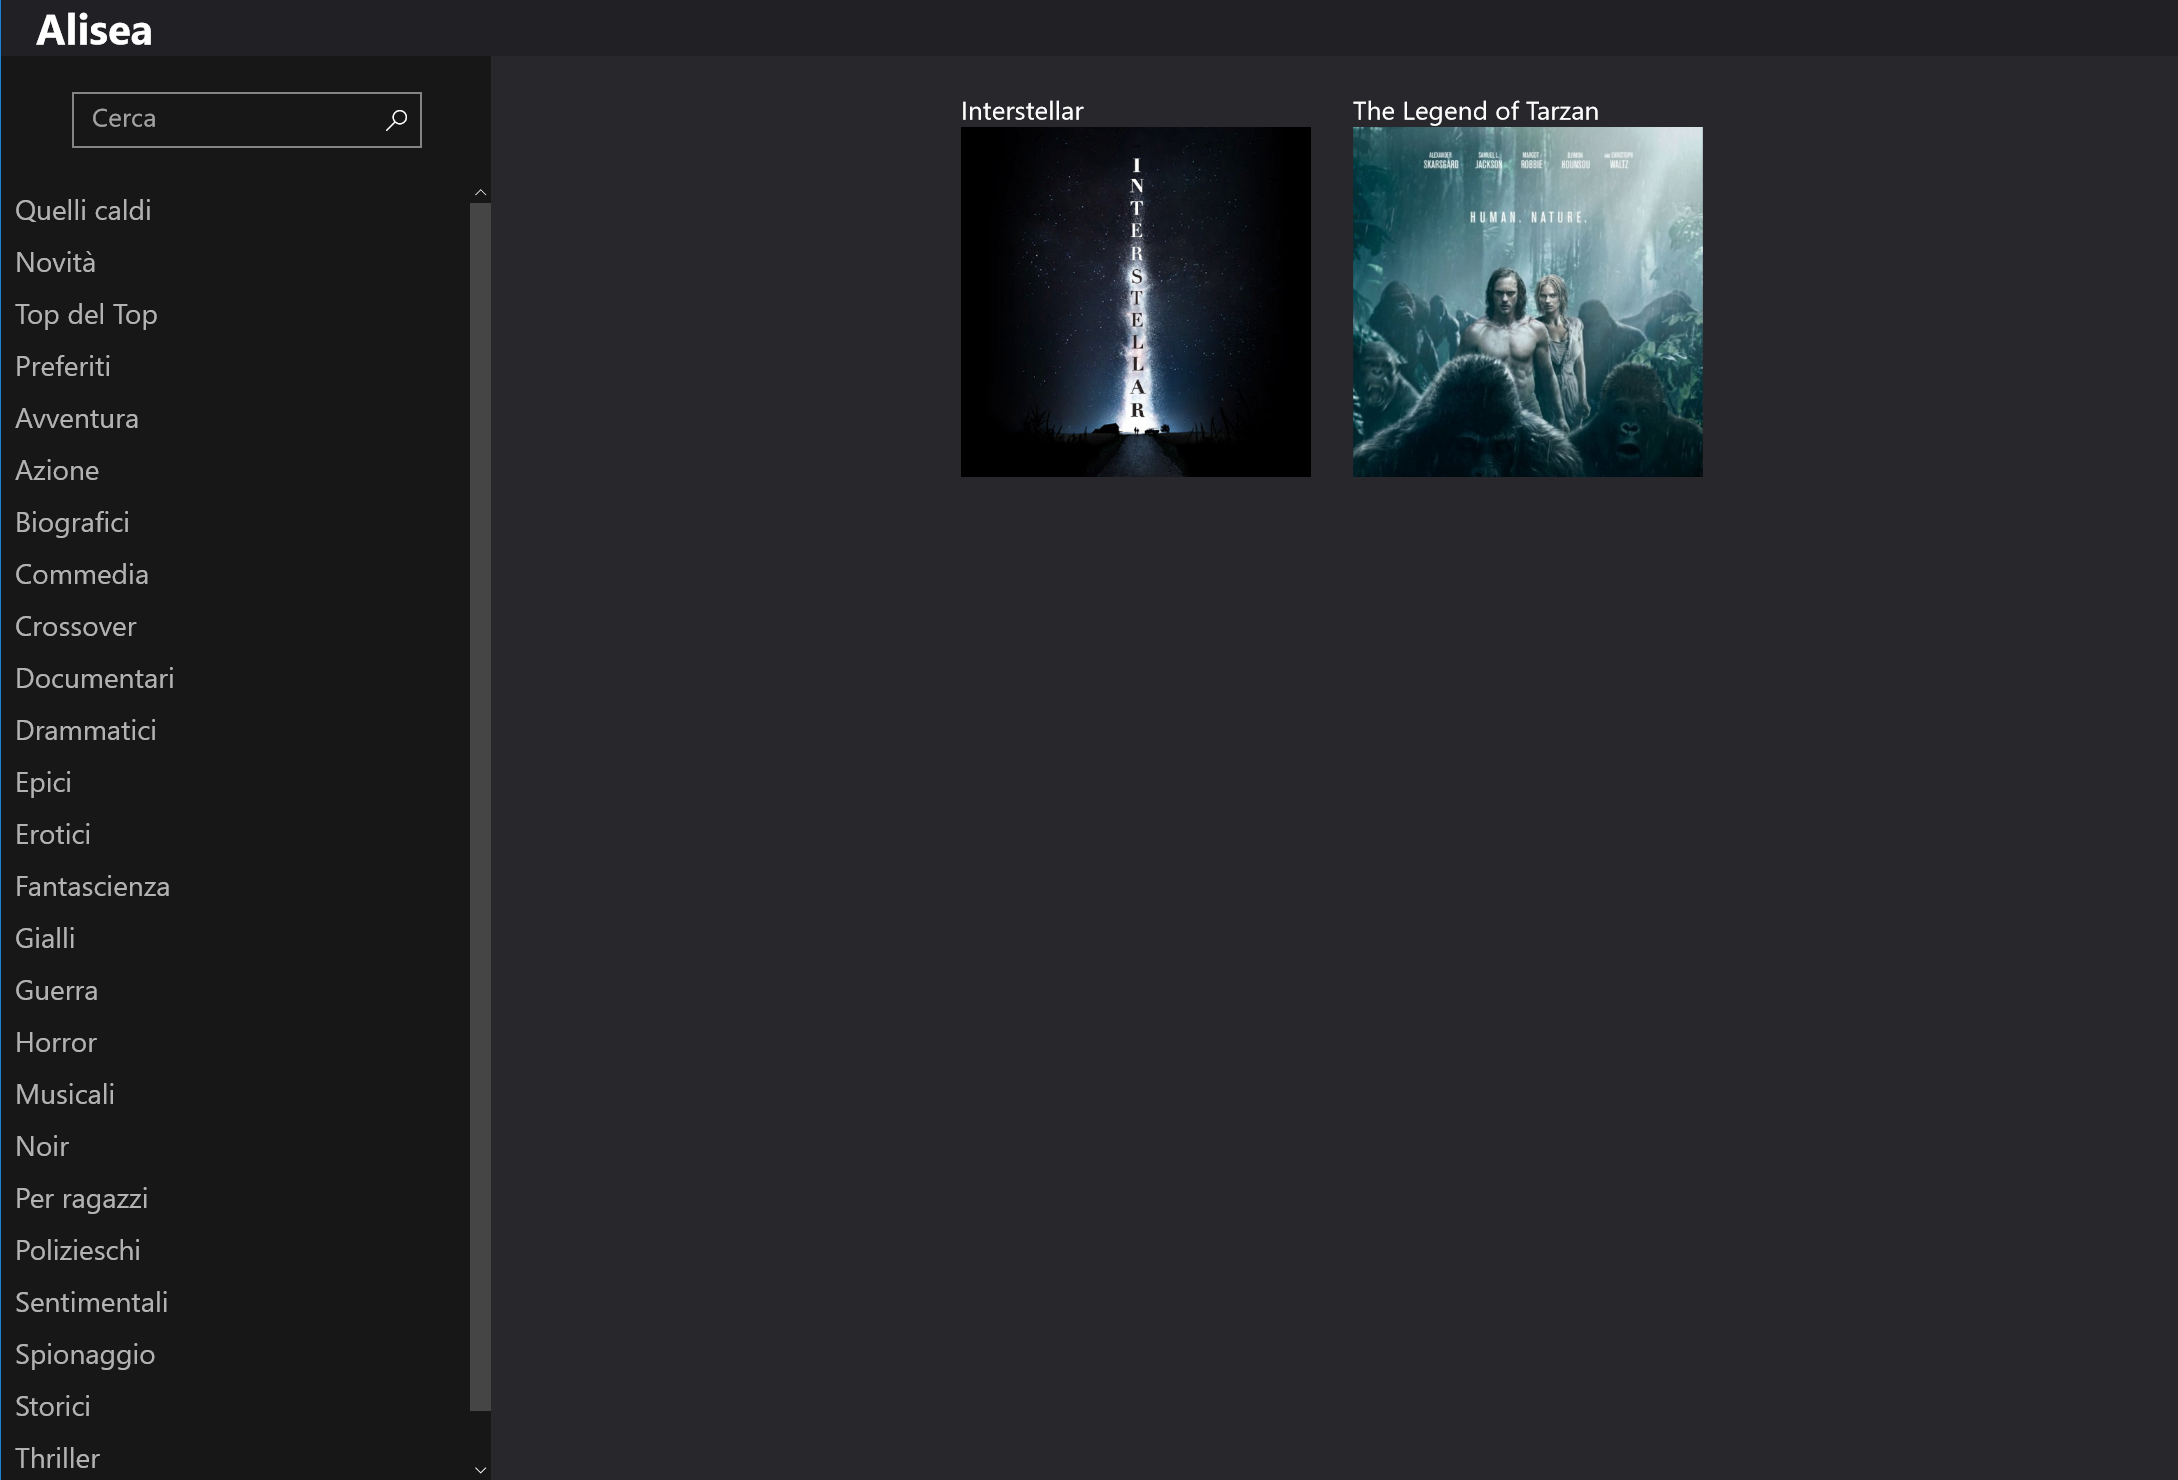
\includegraphics[width=\textwidth]{homepage}
		\caption{Un esempio di homepage dell'applicazione. I film presenti sono per puro scopo espositivo.}
	\end{figure}
\end{center}

\subsection{Pagina dei dettagli del video}
Cliccando sul video sarà possibile accedere alla sua pagina informativa in cui sono presenti diversi elementi, tra cui:
\begin{itemize}
	\item \textbf{Dettagli del video: }è possibile visualizzare la locandina del video, il titolo, la durata, il numero di visualizzazioni, la descrizione ed eventuali attori e reigisti che ne hanno preso parte.
	\item \textbf{Componenti grafici per la valutazione: }è possibile mostrare il proprio apprezzamente o meno cliccando sull'icona raffigurante un pollice rivolto verso l'alto o verso il basso, consentendo anche di poterlo salvare tra i preferiti cliccando invece sull'immagine raffigurante un cuore.
	\item \textbf{Filmati presenti nel torrent: }poichè un torrent di un video può essere composto da più filmati, verranno mostrati tutti i filmati appartenenti ad esso dando la possibilità di visualizzarli mediante un clic su di essi. L'applicazione client Alisea sfrutta la libreria di classi Alisea Torrent per permettere la visualizzazione di tali contenuti multimediali.\\
\end{itemize}
\begin{center}
	\begin{figure}[h!]
		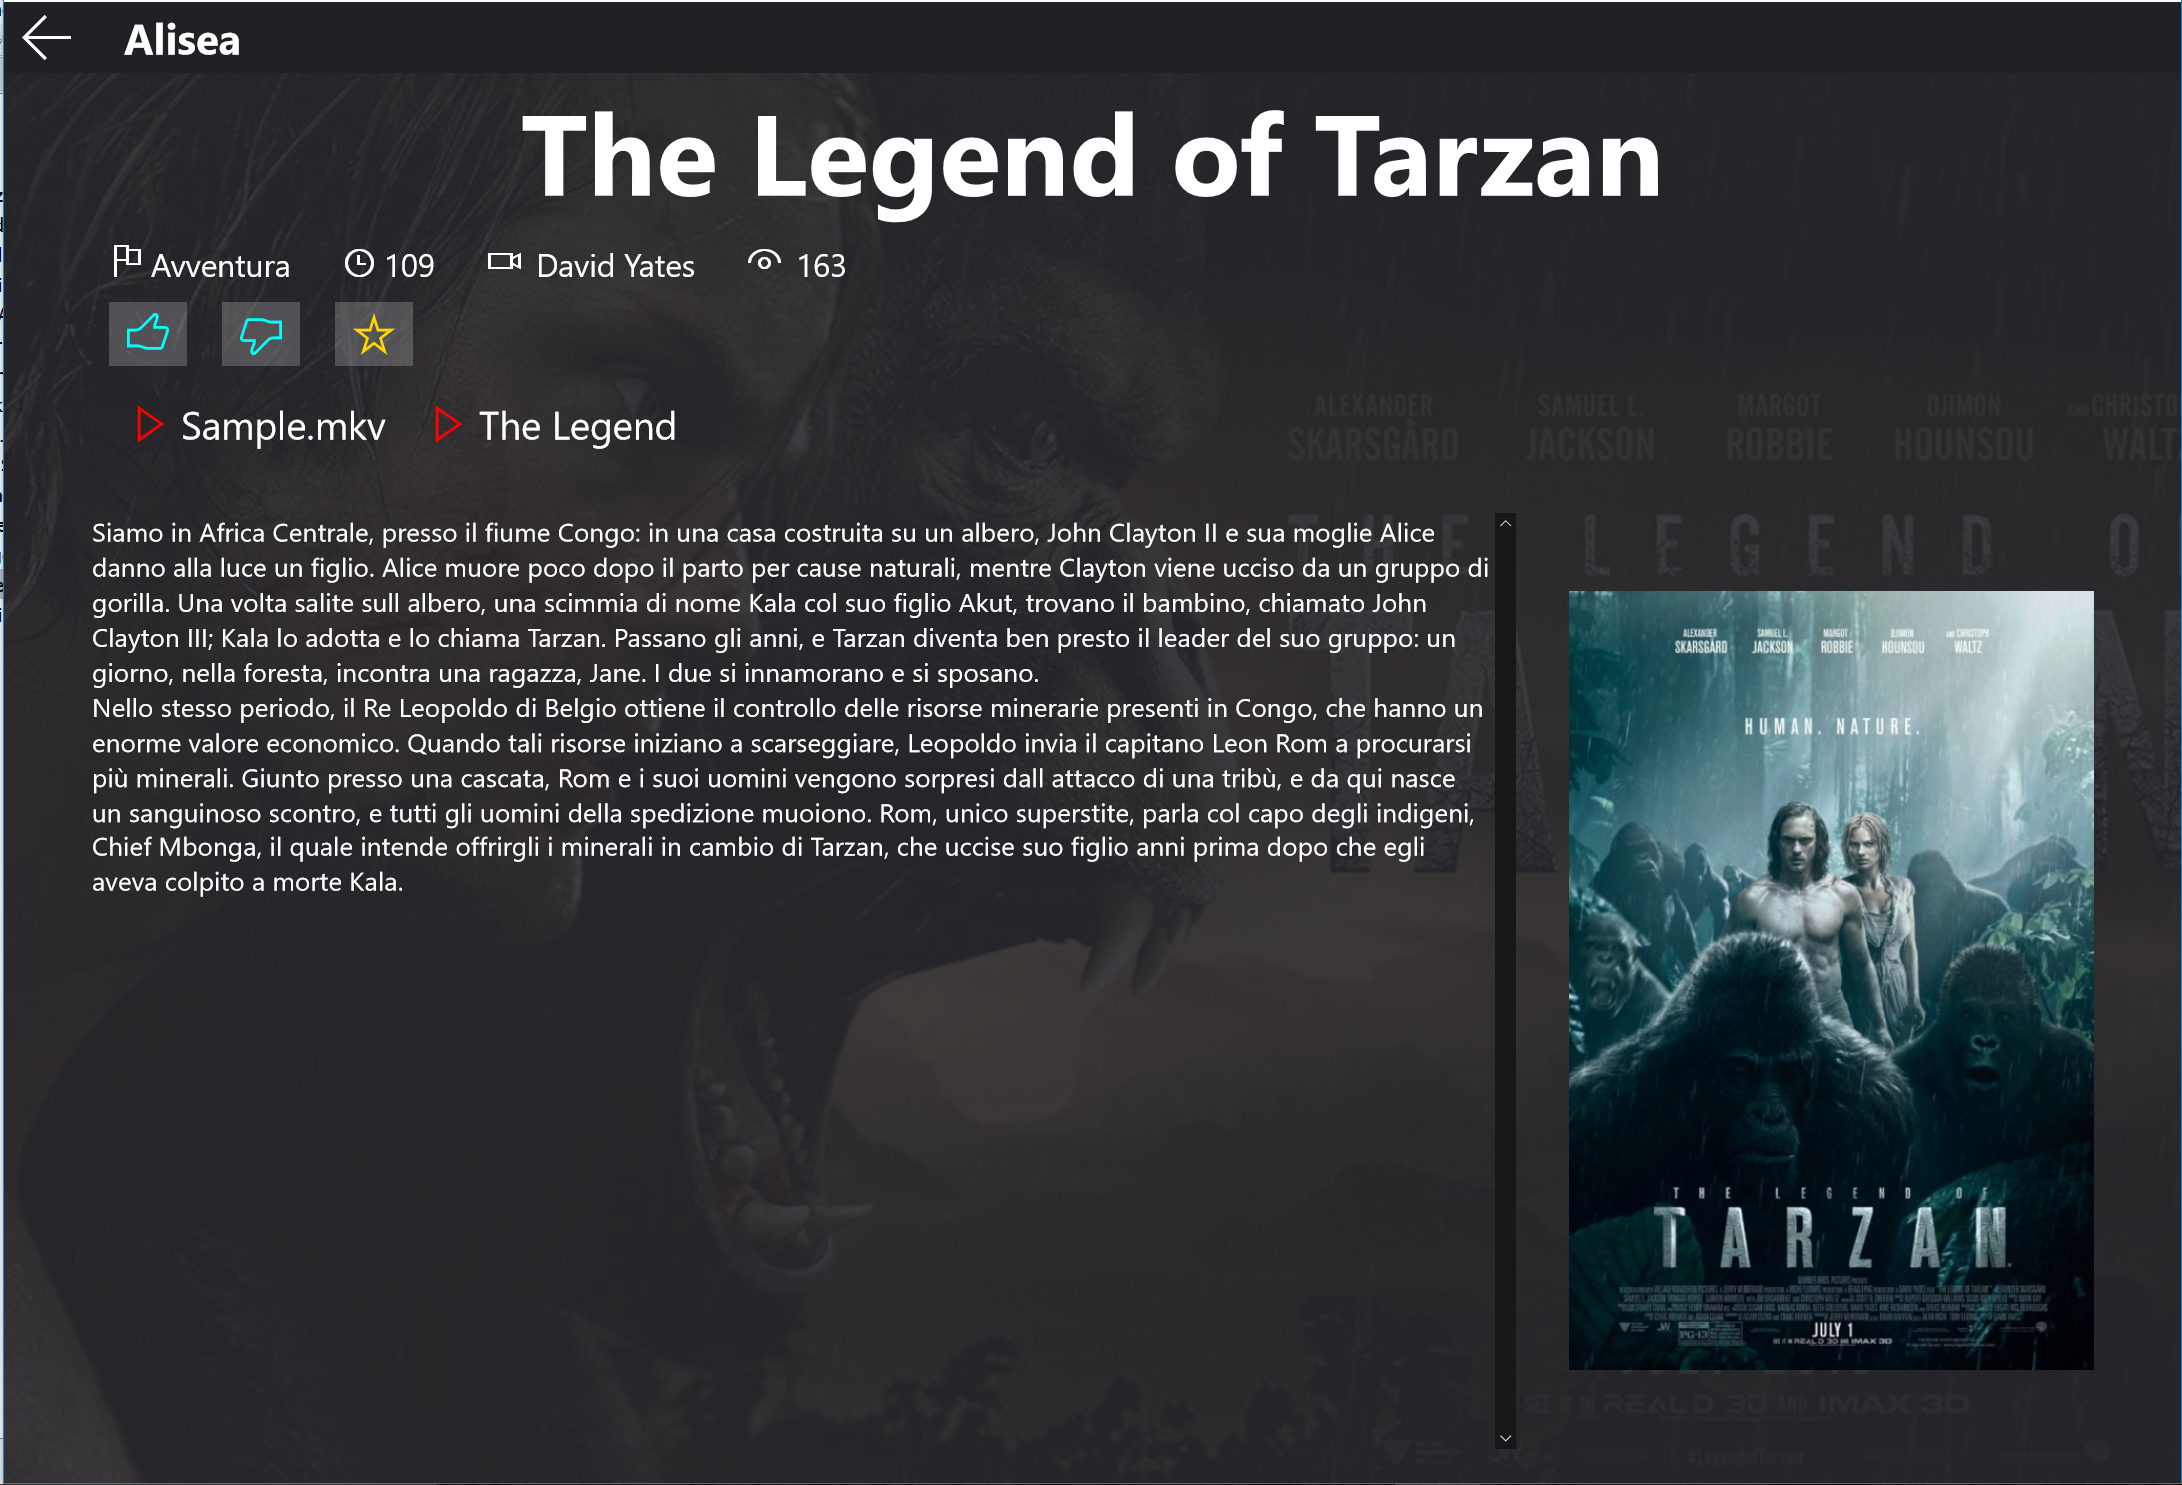
\includegraphics[width=\textwidth]{filmdetail}
		\caption{Un esempio di un torrent raffigurante il film The Legend of Tarzan. Il film in questione è stato utilizzato per puro scopo d'esempio e non è mai stato guardato grazie a questa applicazione.\\}
	\end{figure}
\end{center}
Cliccando su un filmato presente nella pagina dei dettagli l'applicazione partirà con la comunicazione via torrent al fine di ottenere tutte le parti del video in via sequenziale, lanciando un riproduttore per poterlo poi visualizzare.
\newpage
\subsection{Pagina di riproduzione video}
La schermata di riproduzione è accessibile tramite la pagina dei dettagli di un video: tale schermata fornisce i controlli per avviare, mettere in pausa il video e muoversi al suo interno.\newline
Arrivati in questa schermata viene istanziato un oggetto \textit{AliseaCoreTorrent} per iniziare la comunicazione con tracker, peer e per ottenere i dati multimediali da riprodurre.\\
Per fornire i dati al riproduttore multimediale è stata implementata la classe \textit{VideoRandomAccessStream} che rispetta l'interfaccia \textit{IRandomAccessStream}; un'istanza di questa classe viene impostata come sorgente dei dati del lettore multimediale.\\
L'istanza \textit{VideoRandomAccessStream} ottiene dall'oggetto AliseaCoreTorrent un riferimento al Data Store e ogni richiesta dati sopraggiunta dal lettore multimediale viene inoltrata cosi al Data Store.



\chapter{Sviluppi futuri}
L'applicazione attualmente ha la struttura tipica di un prototipo sia dal punto di vista del backend che del frontend, con numerosi margini di implementazione riassumibili dal seguente elenco: \newline

\paragraph{Frontend:} per quanto riguarda il frontend, è possibile:
\begin{itemize}
	\item \textbf{Migliorare la gestione dei dati in memoria}: attualmente i dati vengono mantenuti nella memoria centrale. Questa non è sicuramente la soluzione ottimale. Si può pensare di scriverli su disco o di eliminare i dati meno recenti in caso di memoria limitata.
	\item\textbf{Fornire supporto al protocollo uTP}: il micro Transport Protocol è un protocollo sostitutivo alla comunicazione TCP tra peer. Questo si costruisce sul layer UDP e permette di gestire i congestionamenti del traffico tra peer.
	\item\textbf{Gestione alternativa delle richieste dati}: attualmente le richieste dei pezzi possono causare molto traffico indesiderato. Si può lavorare sui limiti del numero di richieste e provare a mandare messaggi \textit{CancelRequest} ai peer in seguito al completamento dei pezzi.
\end{itemize}

\paragraph{Backend:}per quanto riguarda il backend, è possibile:
\begin{itemize}
	\item \textbf{Implementare un sistema di caching}: mimando una GET condizionale in cui, se il client ha la versione più recente di una certa lista di video, non viene fornito nessun nuovo video abbassando drasticamente il tempo medio di esecuzione.
	\item \textbf{Miglioramento del database}: modificando la struttura secondo un'ottica più vicino alla scalabilità ed inserendo le varie operazioni da effettuare in caso ad esempio di cancellazione di un determinato record o di una relazione.
	\item \textbf{Miglioramento del sito dell'applicazione}: migliorando la qualità della grafica e del contenuto informativo.
	\item \textbf{Effettuare un refactoring della classi DatabaseManager}: rendendo templatica la richiesta al server di una determinata in base alla tipologia di API.
	\item \textbf{Introdurre un database documentale} su cui salvare le immagini e i file .torrent dei video anzichè appoggiarsi su scelte meno performanti come Google Drive ad esempio.
\end{itemize}

\begin{thebibliography}{9}
	
	\bibitem{lamport94}
	Paolo Atzeni, Basi di dati: modelli e linguaggi di interrogazione, Quarta Edizione, McGraw-Hill, 2013
	\bibitem{lamport94}
	Kalen Delaney, SQL Server 2012 Internals, Microsoft, 2012
	\bibitem{lamport94}
	Il logo di Alisea è stato realizzato da Tommaso Pistillo: \url{http://www.tommasopistillo.com/}
	
	\end{thebibliography}
	
\end{document}

